\documentclass[11pt,a4paper]{article}

\usepackage[utf8]{inputenc}
\usepackage[T1]{fontenc}
\usepackage{lmodern}
\usepackage{amsmath,amsthm,amssymb,amsfonts,mathtools}
\usepackage{geometry}
\usepackage{setspace}
\usepackage{fancyhdr}
\usepackage{hyperref}
\usepackage{enumitem}
\usepackage{float}
\usepackage{tikz}
\usepackage{pgfplots}
\pgfplotsset{compat=1.18}
\usetikzlibrary{arrows.meta,patterns,decorations.markings,calc,positioning,shapes.geometric,decorations.pathreplacing,backgrounds,shadings,fit}
\usepackage[ruled,vlined,linesnumbered]{algorithm2e}
\usepackage{xcolor}
\usepackage{academicons}
\usepackage{tcolorbox}
\tcbuselibrary{breakable,skins}
\usepackage{caption}
\usepackage{titlesec}

% ── Color palette ──
\definecolor{accent}{HTML}{2B4C7E}      % deep blue
\definecolor{accentlight}{HTML}{E8EEF6}  % very light blue
\definecolor{thmcolor}{HTML}{1B6B4A}     % dark teal (theorems)
\definecolor{defcolor}{HTML}{7B3F00}     % warm brown (definitions)
\definecolor{excolor}{HTML}{4A4A8A}      % muted indigo (examples)
\definecolor{remcolor}{HTML}{606060}      % neutral gray (remarks)

% ── Section heading style ──
\titleformat{\section}
  {\Large\bfseries\color{accent}}
  {\thesection}{0.8em}{}
  [\vspace{-0.6em}{\color{accent}\rule{\textwidth}{0.6pt}}]
\titleformat{\subsection}
  {\large\bfseries\color{accent!80!black}}
  {\thesubsection}{0.7em}{}

% ── Caption style ──
\captionsetup{
  font=small,
  labelfont={bf,color=accent},
  textfont={color=black!80},
  margin=1em,
}

% ── Repository URL ──
\newcommand{\repourl}{https://github.com/gabayae/expansive-homeomorphisms-complexity-qmetric}

% ── Small margins, small interlines ──
\geometry{a4paper, left=0.85in, right=0.85in, top=1.0in, bottom=0.95in,
          headheight=14pt}

\setstretch{1.08}
\setlength{\parindent}{0em}
\setlength{\parskip}{0.5em}

% ── Running headers/footers ──
\pagestyle{fancy}
\fancyhf{}
\fancyhead[L]{\small\color{accent}\itshape Expansive homeomorphisms on complexity quasi-metric spaces}
\fancyhead[R]{\small\color{accent}\thepage}
\renewcommand{\headrule}{{\color{accent}\hrule width\headwidth height 0.4pt}}
\renewcommand{\footrulewidth}{0pt}

% Title page style (no header)
\fancypagestyle{titlepage}{%
  \fancyhf{}%
  \renewcommand{\headrulewidth}{0pt}%
  \renewcommand{\footrulewidth}{0pt}%
}


% ── Highlighted box for key insights ──
\newtcolorbox{insightbox}[1][]{
  colback=accent!4,
  colframe=accent,
  fonttitle=\bfseries,
  title={#1},
  boxrule=0.5pt,
  arc=3pt,
  breakable,
  left=6pt, right=6pt,
}

\newtcolorbox{keyresult}[1][]{
  colback=thmcolor!4,
  colframe=thmcolor,
  fonttitle=\bfseries\color{thmcolor},
  title={#1},
  boxrule=0.5pt,
  arc=3pt,
}

% ── Theorem environments (with subtle left-bar styling) ──
\theoremstyle{plain}
\newtheorem{theoreminner}{Theorem}[section]
\newtheorem{lemmainner}[theoreminner]{Lemma}
\newtheorem{propositioninner}[theoreminner]{Proposition}
\newtheorem{corollaryinner}[theoreminner]{Corollary}
\theoremstyle{definition}
\newtheorem{definitioninner}[theoreminner]{Definition}
\newtheorem{exampleinner}[theoreminner]{Example}
\newtheorem{remarkinner}[theoreminner]{Remark}

% Wrap each in a tcolorbox with a colored left bar
\tcolorboxenvironment{theoreminner}{
  blanker, breakable,
  left=4pt, borderline west={2.5pt}{0pt}{thmcolor},
  before skip=8pt, after skip=8pt,
}
\tcolorboxenvironment{lemmainner}{
  blanker, breakable,
  left=4pt, borderline west={2.5pt}{0pt}{thmcolor!70},
  before skip=8pt, after skip=8pt,
}
\tcolorboxenvironment{propositioninner}{
  blanker, breakable,
  left=4pt, borderline west={2.5pt}{0pt}{thmcolor!70},
  before skip=8pt, after skip=8pt,
}
\tcolorboxenvironment{corollaryinner}{
  blanker, breakable,
  left=4pt, borderline west={2.5pt}{0pt}{thmcolor!50},
  before skip=8pt, after skip=8pt,
}
\tcolorboxenvironment{definitioninner}{
  blanker, breakable,
  left=4pt, borderline west={2.5pt}{0pt}{defcolor},
  before skip=8pt, after skip=8pt,
}
\tcolorboxenvironment{exampleinner}{
  blanker, breakable,
  left=4pt, borderline west={2pt}{0pt}{excolor!60},
  before skip=8pt, after skip=8pt,
}
\tcolorboxenvironment{remarkinner}{
  blanker, breakable,
  left=4pt, borderline west={1.5pt}{0pt}{remcolor!40},
  before skip=6pt, after skip=6pt,
}

% Light gray box for proofs
\tcolorboxenvironment{proof}{
  colback=black!3,
  colframe=black!15,
  boxrule=0.4pt,
  arc=2pt,
  breakable,
  left=6pt, right=6pt, top=4pt, bottom=4pt,
  before skip=8pt, after skip=8pt,
}

% Aliases so the rest of the document uses the same names
\newenvironment{theorem}[1][]{\begin{theoreminner}[#1]}{\end{theoreminner}}
\newenvironment{lemma}[1][]{\begin{lemmainner}[#1]}{\end{lemmainner}}
\newenvironment{proposition}[1][]{\begin{propositioninner}[#1]}{\end{propositioninner}}
\newenvironment{corollary}[1][]{\begin{corollaryinner}[#1]}{\end{corollaryinner}}
\newenvironment{definition}[1][]{\begin{definitioninner}[#1]}{\end{definitioninner}}
\newenvironment{example}[1][]{\begin{exampleinner}[#1]}{\end{exampleinner}}
\newenvironment{remark}[1][]{\begin{remarkinner}[#1]}{\end{remarkinner}}

\newcommand{\R}{\mathbb{R}}
\newcommand{\N}{\mathbb{N}}
\newcommand{\Z}{\mathbb{Z}}
\newcommand{\Q}{\mathbb{Q}}
\newcommand{\C}{\mathcal{C}}
\newcommand{\BigO}{\mathcal{O}}
\newcommand{\eps}{\varepsilon}
\newcommand{\orb}{\mathrm{orb}}

\hypersetup{
    colorlinks=true,
    linkcolor=accent,
    citecolor=thmcolor,
    urlcolor=excolor,
    hypertexnames=false
}

\begin{document}

% ═══════════════════════════════════════════════════════════════
%  TITLE PAGE
% ═══════════════════════════════════════════════════════════════
\pagenumbering{Alph}
\begin{titlepage}
\thispagestyle{titlepage}
\centering
\vspace*{0.6cm}

{\color{accent}\rule{0.4\textwidth}{0.8pt}}

\vspace{0.8cm}

{\huge\bfseries\color{accent} Expansive homeomorphisms on\\[0.5em]
 complexity quasi-metric spaces}

\vspace{0.5cm}
{\Large\itshape\color{accent!70!black} A bridge between dynamical systems\\[0.2em]
 and computational complexity theory}

\vspace{0.3cm}
{\color{accent}\rule{0.25\textwidth}{0.5pt}}

\vspace{0.8cm}

{\large
\textbf{Ya\'e U.\ Gaba}$^{\dagger,\ddagger,\S}$
}

\vspace{0.3cm}

{\normalsize\color{red!70!black}
\href{https://orcid.org/0000-0001-8128-9704}{\aiOrcid}%
\enspace
\href{https://arxiv.org/a/gaba_y_1.html}{\aiarXiv}%
\enspace
\href{https://scholar.google.com/citations?user=UTszjV4AAAAJ&hl=en}{\aiGoogleScholar}%
}

\vspace{0.5cm}

{\small
$^{\dagger}$\,AI Research and Innovation Nexus for Africa (AIRINA Labs),
AI.Technipreneurs, B\'enin\\[0.3em]
$^{\ddagger}$\,Sefako Makgatho Health Sciences University (SMU),
South Africa\\[0.3em]
$^{\S}$\,African Center for Advanced Studies (ACAS), Cameroon
}

\vspace{1.5cm}
\begin{abstract}
\noindent
The complexity quasi-metric, introduced by Schellekens,
provides a topological framework where the asymmetric nature of
computational comparisons---stating that one algorithm is faster than
another carries different information than stating the second is slower
than the first---finds precise mathematical expression.
In this paper we develop a comprehensive theory of expansive
homeomorphisms on complexity quasi-metric spaces.
Our central result establishes that the scaling transformation
$\psi_\alpha(f)(n)=\alpha f(n)$ is expansive on the complexity space
$(\C,d_\C)$ if and only if $\alpha\neq 1$.
The $\delta$-stable sets arising from this dynamics correspond exactly
to asymptotic complexity classes, providing a dynamical characterisation
of fundamental objects in complexity theory.
We prove that the canonical coordinates associated with $\psi_\alpha$
are hyperbolic with contraction rate $\lambda=1/\alpha$ and establish
a precise connection between orbit separation in the dynamical system
and the classical time hierarchy theorem of Hartmanis and Stearns.
We further investigate unstable sets, conjugate dynamics, and
topological entropy estimates for the scaling map.
Throughout, concrete algorithms and Python implementations accompany
the proofs, making every result computationally reproducible.
SageMath verification snippets are inlined alongside the examples,
and the full code is available in the companion repository.

\medskip
\textbf{Keywords:} Expansive homeomorphism; complexity quasi-metric;
computational complexity; asymmetric topology; dynamical systems;
stable and unstable sets; canonical coordinates

\smallskip
\textbf{2020 MSC:} 54H20; 37B20; 68Q25; 54E35
\end{abstract}
\vfill
\end{titlepage}
\pagenumbering{arabic}

\vspace*{0.5cm}
\begin{flushright}
\begin{minipage}{0.72\textwidth}
\raggedleft\itshape\color{accent!80!black}
``The study of iteration, the study of the behaviour of a transformation
when it is repeated, is the fundamental problem of dynamics.''
\vspace{0.3em}

\upshape\color{accent!60!black}--- Henri Poincar\'e
\end{minipage}
\end{flushright}
\vspace{0.8cm}

% ═══════════════════════════════════════════════════════════════
\section{Introduction: where dynamics meets computation}
\label{sec:intro}
% ═══════════════════════════════════════════════════════════════

\subsection{A tale of two theories}

Mathematics draws much of its power from unexpected bridges between
seemingly distant subjects.  Fourier analysis connects the study of
heat flow to number theory; ergodic theory links statistical mechanics
to measure-preserving transformations; and category theory reveals
shared structure across algebra, topology, and logic.  This paper
explores another such bridge: between \emph{dynamical systems}---the
study of how systems evolve over time---and \emph{computational
complexity theory}---the study of the intrinsic difficulty of
computational problems.

At first glance these two fields appear to have little in common.
Dynamical systems theory asks: given a map $\psi\colon X\to X$,
how do the orbits $\{x,\psi(x),\psi^2(x),\ldots\}$ behave as the
number of iterations grows?  Do nearby orbits stay close, or do they
diverge?  If they diverge, how quickly?  Complexity theory, on the
other hand, asks: given a computational problem, how do the resources
required to solve it---time, memory, communication---grow with the
input size~$n$?

The key observation that connects these two worlds is that
\emph{complexity comparisons are inherently asymmetric}.  Saying
``algorithm~$A$ is at most as fast as algorithm~$B$'' is not the
same as saying ``algorithm~$B$ is at most as slow as algorithm~$A$.''
More precisely, if $f(n)\le g(n)$ for all~$n$ (so that $f$~is at
least as fast as~$g$), the ``cost'' of moving from $f$ to~$g$ in the
complexity landscape is zero---we are moving to a slower algorithm,
which is easy to simulate---but the cost of moving from $g$ to~$f$ is
positive, because improving an algorithm's running time requires
genuine insight.

This asymmetry is captured perfectly by the mathematical notion of a
\emph{quasi-metric}: a distance function $q$ where $q(x,y)$ need not
equal $q(y,x)$.  Schellekens~\cite{schellekens1995} introduced the
\emph{complexity quasi-metric} $d_\C$ on the space of functions
$f\colon\N\to(0,\infty)$ and showed that its topological properties
encode fundamental features of computational complexity.  Romaguera
and Schellekens~\cite{romaguera1999} subsequently developed the
quasi-metric structure of complexity spaces in depth.

On the dynamical side, \emph{expansive homeomorphisms}---maps under
which every pair of distinct points is eventually separated by more
than some fixed threshold~$\delta$---are a central object of study,
going back to Utz~\cite{utz1950} and developed extensively by
Bowen~\cite{bowen1975} and Reddy~\cite{reddy1983}.  Recently, Olela
Otafudu, Matladi, and Zweni~\cite{olela2024} extended the theory of
expansive homeomorphisms to quasi-metric spaces, opening the door to
applications in asymmetric settings.

Our contribution is to walk through that door and apply the theory of
expansive homeomorphisms to the complexity quasi-metric space.  The
results reveal that basic dynamical concepts---orbits, stable sets,
hyperbolicity---have direct and illuminating counterparts in
complexity theory.

\paragraph{Related work.}
The complexity quasi-metric space was introduced by
Schellekens~\cite{schellekens1995}, who established its basic
topological properties and connections to denotational semantics.
Romaguera and Schellekens~\cite{romaguera1999} subsequently
developed the quasi-metric structure in depth, proving
completeness results and studying the Smyth completion.  On
the dynamical side, expansive homeomorphisms on metric spaces
have a long history, beginning with Utz~\cite{utz1950} and
substantially advanced by Bowen~\cite{bowen1975}, who connected
expansiveness to topological entropy, and Reddy~\cite{reddy1983},
who established canonical coordinate systems for expansive maps.
The extension of expansive homeomorphisms to quasi-metric spaces
was carried out by Olela Otafudu, Matladi, and
Zweni~\cite{olela2024}, who proved that $q$-expansiveness and
$q^t$-expansiveness are equivalent and developed the abstract
theory of stable and unstable sets in the asymmetric setting.
K\"unzi~\cite{kunzi1995,kunzi2001} provided a comprehensive
account of the topology of quasi-metric spaces, which underpins
the present work.

The novelty of our approach lies in the \emph{combination} of
these two lines of research: whereas~\cite{olela2024} develops
the abstract theory without a specific quasi-metric space in mind,
and~\cite{schellekens1995,romaguera1999} study the complexity
space without dynamical-systems tools, we bring the two together
and show that the resulting interplay yields concrete insights
in both directions---dynamical concepts acquire computational
meaning, and complexity-theoretic distinctions acquire dynamical
characterisations.

\begin{figure}[H]
\centering
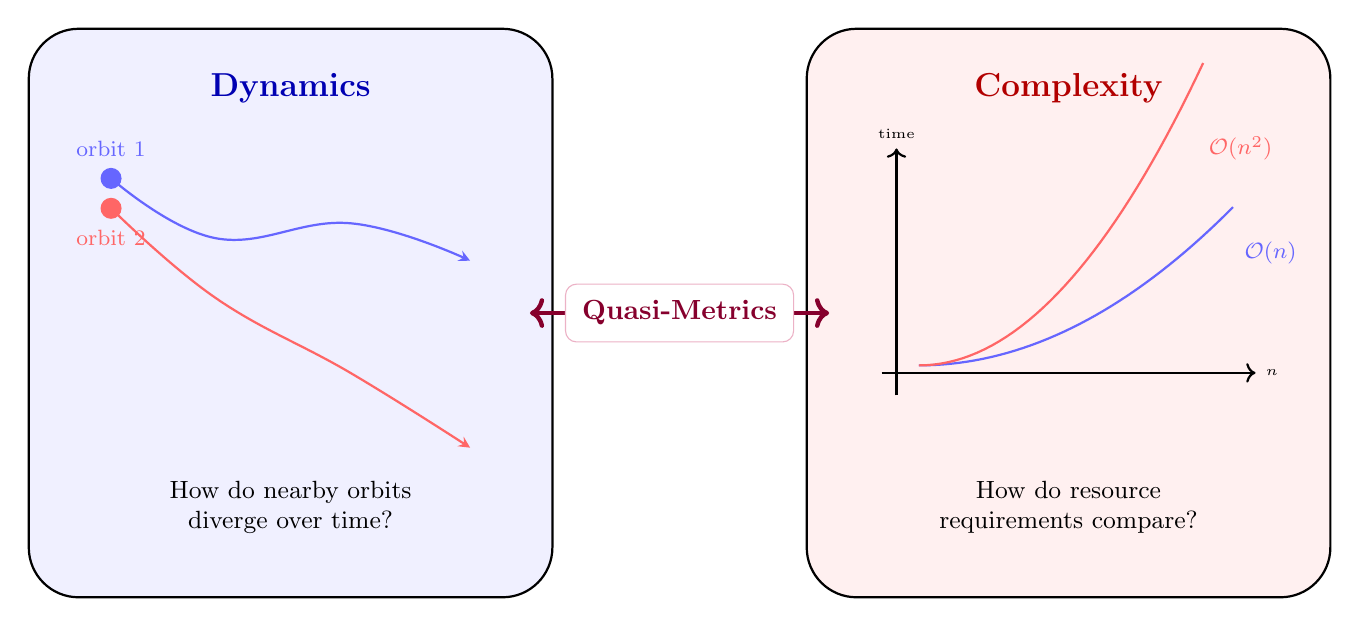
\begin{tikzpicture}[scale=0.95]
    % Dynamics box
    \begin{scope}[shift={(-5.2,0)}]
        \draw[thick, fill=blue!6, rounded corners=18pt]
             (-3.5,-3.8) rectangle (3.5,3.8);
        \node[font=\large\bfseries, blue!70!black] at (0,3.0) {Dynamics};
        \draw[thick, blue!60, ->, >=stealth]
             plot[smooth, tension=0.7]
             coordinates {(-2.4,1.8) (-1.0,1.0) (0.8,1.2) (2.4,0.7)};
        \draw[thick, red!60, ->, >=stealth]
             plot[smooth, tension=0.7]
             coordinates {(-2.4,1.4) (-1.0,0.2) (0.8,-0.8) (2.4,-1.8)};
        \fill[blue!60] (-2.4,1.8) circle (4pt);
        \fill[red!60]  (-2.4,1.4) circle (4pt);
        \node[font=\footnotesize, blue!60] at (-2.4,2.2) {orbit 1};
        \node[font=\footnotesize, red!60] at (-2.4,1.0) {orbit 2};
        \node[font=\small, text width=4.5cm, align=center]
             at (0,-2.6) {How do nearby orbits\\diverge over time?};
    \end{scope}
    % Complexity box
    \begin{scope}[shift={(5.2,0)}]
        \draw[thick, fill=red!6, rounded corners=18pt]
             (-3.5,-3.8) rectangle (3.5,3.8);
        \node[font=\large\bfseries, red!70!black] at (0,3.0) {Complexity};
        \draw[thick, ->] (-2.5,-0.8) -- (2.5,-0.8) node[right, font=\tiny] {$n$};
        \draw[thick, ->] (-2.3,-1.1) -- (-2.3,2.2) node[above, font=\tiny] {time};
        \draw[thick, blue!60, domain=-2.0:2.2, samples=40]
             plot (\x, {0.12*(\x+2)*(\x+2) - 0.7});
        \draw[thick, red!60, domain=-2.0:1.8, samples=40]
             plot (\x, {0.28*(\x+2)*(\x+2) - 0.7});
        \node[font=\footnotesize, blue!60]  at (2.7, 0.8) {$\BigO(n)$};
        \node[font=\footnotesize, red!60]   at (2.3, 2.2) {$\BigO(n^2)$};
        \node[font=\small, text width=4.5cm, align=center]
             at (0,-2.6) {How do resource\\requirements compare?};
    \end{scope}
    % Connecting arrow
    \draw[ultra thick, <->, purple!70!black] (-2.0,0) -- (2.0,0);
    \node[font=\bfseries, purple!70!black, fill=white, inner sep=6pt,
          rounded corners=4pt, draw=purple!30]
         at (0,0) {Quasi-Metrics};
\end{tikzpicture}
\caption{Two worlds connected by quasi-metrics.  Dynamical systems study
orbit divergence; complexity theory studies resource growth.  The
asymmetry inherent in both settings is encoded by the quasi-metric
distance.}
\label{fig:two-worlds}
\end{figure}


\subsection{Why quasi-metrics?}

Before we proceed, let us briefly motivate why quasi-metrics---rather
than ordinary metrics---are the right tool for this investigation.

In a standard metric space $(X,d)$, the symmetry axiom $d(x,y)=d(y,x)$
ensures that the cost of moving from~$x$ to~$y$ is the same as the
cost of moving from~$y$ to~$x$.  This is natural in many geometric
settings, but it is \emph{unnatural} in computational settings.  Consider
two algorithms with running times $f(n)=n$ and $g(n)=n^2$.  Given
the faster algorithm~$f$, one can trivially simulate the slower
algorithm~$g$ by wasting time.  But given the slower algorithm~$g$,
one cannot in general produce the faster algorithm~$f$ without effort.
The ``distance'' from fast to slow should therefore be zero (or small),
while the distance from slow to fast should be positive.

This is exactly what a quasi-metric provides.  By dropping the symmetry
axiom, quasi-metrics can encode directional costs, and the complexity
quasi-metric $d_\C$ does precisely this: $d_\C(f,g)=0$ whenever
$f(n)\le g(n)$ for all~$n$ (fast to slow is free), while
$d_\C(g,f)>0$ when $g$ is genuinely slower (slow to fast is costly).

\begin{figure}[H]
\centering
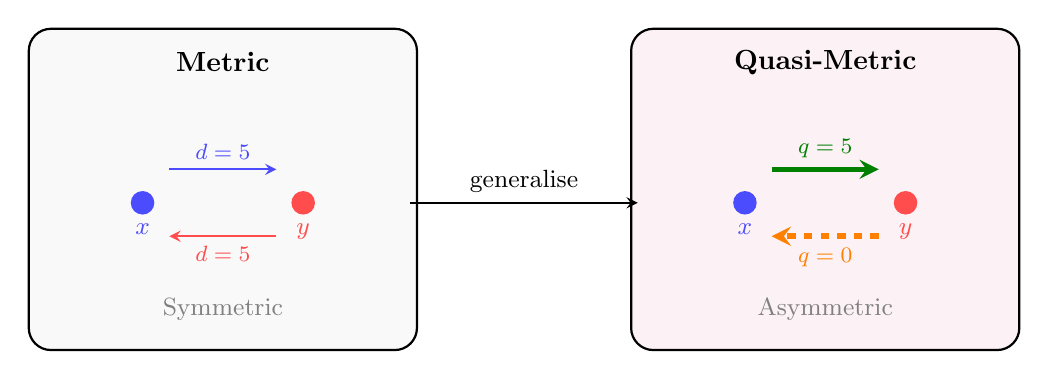
\begin{tikzpicture}[scale=0.85, >=stealth]
  % Metric world
  \begin{scope}[shift={(-4.5,0)}]
    \draw[thick, rounded corners=8pt, fill=gray!5] (-2.9,-2.2) rectangle (2.9,2.6);
    \node[font=\bfseries] at (0,2.1) {Metric};
    \fill[blue!70] (-1.2,0) circle (5pt) node[below=4pt, font=\small] {$x$};
    \fill[red!70]  (1.2,0) circle (5pt) node[below=4pt, font=\small] {$y$};
    \draw[thick, blue!70, ->] (-0.8,0.5) -- (0.8,0.5)
      node[midway, above, font=\footnotesize] {$d=5$};
    \draw[thick, red!70, ->] (0.8,-0.5) -- (-0.8,-0.5)
      node[midway, below, font=\footnotesize] {$d=5$};
    \node[font=\small, gray] at (0,-1.6) {Symmetric};
  \end{scope}
  % Quasi-metric world
  \begin{scope}[shift={(4.5,0)}]
    \draw[thick, rounded corners=8pt, fill=purple!5] (-2.9,-2.2) rectangle (2.9,2.6);
    \node[font=\bfseries] at (0,2.1) {Quasi-Metric};
    \fill[blue!70] (-1.2,0) circle (5pt) node[below=4pt, font=\small] {$x$};
    \fill[red!70]  (1.2,0) circle (5pt) node[below=4pt, font=\small] {$y$};
    \draw[very thick, green!50!black, ->, line width=2.0pt] (-0.8,0.5) -- (0.8,0.5)
      node[midway, above, font=\footnotesize] {$q=5$};
    \draw[very thick, orange, ->, dashed, line width=2.0pt] (0.8,-0.5) -- (-0.8,-0.5)
      node[midway, below, font=\footnotesize] {$q=0$};
    \node[font=\small, gray] at (0,-1.6) {Asymmetric};
  \end{scope}
  \draw[thick, ->] (-1.7,0) -- (1.7,0) node[midway, above, font=\small] {generalise};
\end{tikzpicture}
\caption{From metrics to quasi-metrics.  Dropping symmetry allows the
distance to encode directional information.}
\label{fig:metric-vs-quasi}
\end{figure}


\subsection{Overview of main results}

We now give a roadmap of the paper and preview our main contributions.
The reader may find it helpful to refer back to this summary as the
technical details unfold.

Our first result characterises exactly when the scaling transformation
is expansive.

\begin{keyresult}[Theorem~\ref{thm:main-scaling}: Expansiveness of scaling]
The scaling map $\psi_\alpha(f)(n)=\alpha f(n)$ is expansive on the
complexity space $(\C,d_\C)$ if and only if $\alpha\neq 1$.
\end{keyresult}

Our second result reveals that the stable sets of this dynamics have a
beautiful complexity-theoretic interpretation.

\begin{keyresult}[Theorem~\ref{thm:stable-sets}: Stable sets are complexity classes]
For $\alpha>1$, the $\delta$-stable set of $f$ under $\psi_\alpha$
coincides with the set $\{g: d_\C(f,g)\le\delta\}$, which contains
all functions $g$ with $g(n)\ge f(n)$ for every~$n$.
\end{keyresult}

Our third result establishes a precise form of hyperbolicity.

\begin{keyresult}[Theorem~\ref{thm:hyperbolicity}: Hyperbolic canonical coordinates]
The canonical coordinates of $\psi_\alpha$ ($\alpha>1$) exhibit
exponential contraction with rate $\lambda=1/\alpha$ and constant $C=1$.
\end{keyresult}

Our fourth result connects the dynamical picture to a classical theorem
in complexity theory.

\begin{keyresult}[Theorem~\ref{thm:hierarchy}: Hierarchy as orbit separation]
If $f(n)\log f(n)=o(g(n))$, then the orbits of $f$ and $g$ under
$\psi_\alpha$ separate in the symmetrized quasi-metric beyond every
threshold.
\end{keyresult}

Each of these results is proved in detail and accompanied by an
algorithm and a Python implementation.  All code is available in
the companion repository.

\subsection{Organisation}

The paper is organised as follows.  Section~\ref{sec:quasi-metric}
recalls the basic theory of quasi-metric spaces, with examples and
motivation.  Section~\ref{sec:complexity-space} introduces the
complexity quasi-metric of Schellekens and establishes its
fundamental properties, including several illustrative computations.
Section~\ref{sec:expansive} defines expansive homeomorphisms in the
quasi-metric setting.  Section~\ref{sec:scaling} introduces the
scaling transformation and proves our main expansiveness result.
Section~\ref{sec:stable-unstable} develops the theory of stable and
unstable sets.  Section~\ref{sec:hyperbolicity} establishes
hyperbolicity.  Section~\ref{sec:hierarchy} connects orbit
separation to the time hierarchy theorem.
Section~\ref{sec:entropy} discusses topological entropy estimates.
Section~\ref{sec:conclusion} summarises the results and poses open
problems.  All Python implementations and SageMath verification
scripts are available in the companion repository
(\href{\repourl/tree/main/code}{\texttt{code/}} directory).


% ═══════════════════════════════════════════════════════════════
\section{Quasi-metric spaces}
\label{sec:quasi-metric}
% ═══════════════════════════════════════════════════════════════

We begin by recalling the foundational notion of a quasi-metric space.
The theory of quasi-metric spaces has a long history, with major
contributions by K\"unzi~\cite{kunzi1995, kunzi2001},
Cobza\c{s}~\cite{cobzas2013}, and many others.  We follow the
notation and conventions of Olela Otafudu et
al.~\cite{olela2024}.

\begin{definition}[Quasi-metric]\label{def:quasi-metric}
Let $X$ be a non-empty set.  A function
$q\colon X\times X\to[0,\infty)$ is a \emph{quasi-metric} on $X$
if it satisfies the following three axioms for all $x,y,z\in X$:
\begin{enumerate}[label=\textup{(Q\arabic*)},leftmargin=3em]
    \item $q(x,x)=0$; \label{Q1}
    \item $q(x,z)\le q(x,y)+q(y,z)$ \quad(triangle inequality); \label{Q2}
    \item $q(x,y)=0=q(y,x)\;\Rightarrow\;x=y$
      \quad($T_0$~separation). \label{Q3}
\end{enumerate}
The pair $(X,q)$ is called a \emph{quasi-metric space}.
\end{definition}

Notice that the only axiom ``missing'' compared with a metric is
symmetry: we do \emph{not} require $q(x,y)=q(y,x)$.  This single
change opens up a surprisingly rich theory.

Every quasi-metric $q$ gives rise to two natural companions.

\begin{definition}[Conjugate and symmetrization]\label{def:conjugate}
Let $(X,q)$ be a quasi-metric space.  The \emph{conjugate
quasi-metric} is $q^t(x,y):=q(y,x)$.  The \emph{symmetrization} is
$q^s(x,y):=\max\{q(x,y),q^t(x,y)\}=\max\{q(x,y),q(y,x)\}$.
\end{definition}

It is straightforward to verify that $q^t$ is again a quasi-metric
and that $q^s$ is a genuine metric on~$X$.  Thus every quasi-metric
space carries a canonical metric, obtained by taking the ``worst-case
direction'' of the asymmetric distance.

\begin{example}[Standard quasi-metric on $\R$]\label{ex:standard-qm}
Define $u\colon\R\times\R\to[0,\infty)$ by
\[
  u(x,y) \;=\; (y-x)^+ \;=\; \max\{0,\,y-x\}.
\]
Then $u$ is a quasi-metric:  \ref{Q1}~is immediate; \ref{Q2}~follows
from $(z-x)^+\le(y-x)^++(z-y)^+$; and \ref{Q3}~holds because
$u(x,y)=0=u(y,x)$ gives $y\le x$ and $x\le y$, hence $x=y$.

The conjugate is $u^t(x,y)=(x-y)^+$, and the symmetrization is
$u^s(x,y)=|x-y|$, the usual absolute-value metric.
\end{example}

The quasi-metric~$u$ has a vivid interpretation: \emph{going uphill
costs effort, while going downhill is free.}

\begin{figure}[H]
\centering
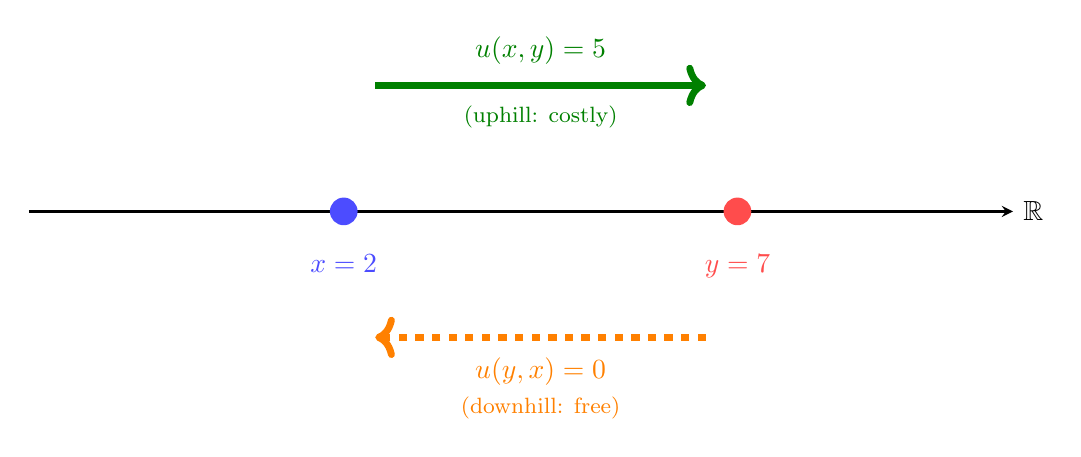
\begin{tikzpicture}[scale=1.0]
    \draw[thick, ->, >=stealth] (-2.0,0) -- (10.5,0) node[right] {$\R$};
    % Tick marks
    \foreach \x in {2, 7} {
      \draw (\x,0.15) -- (\x,-0.15);
    }
    \fill[blue!70]  (2,0) circle (5pt);
    \node[below=12pt, blue!70, font=\bfseries] at (2,0) {$x=2$};
    \fill[red!70]   (7,0) circle (5pt);
    \node[below=12pt, red!70, font=\bfseries]  at (7,0) {$y=7$};
    % Forward arrow (uphill) -- moved higher
    \draw[->, very thick, green!50!black, line width=2.5pt]
         (2.4,1.6) -- (6.6,1.6);
    \node[above=4pt, green!50!black, font=\bfseries] at (4.5,1.6)
         {$u(x,y)=5$};
    \node[below=4pt, green!50!black, font=\footnotesize] at (4.5,1.6)
         {(uphill: costly)};
    % Backward arrow (downhill) -- moved lower
    \draw[->, very thick, orange, dashed, line width=2.5pt]
         (6.6,-1.6) -- (2.4,-1.6);
    \node[below=4pt, orange, font=\bfseries] at (4.5,-1.6)
         {$u(y,x)=0$};
    \node[below=18pt, orange, font=\footnotesize] at (4.5,-1.6)
         {(downhill: free)};
\end{tikzpicture}
\caption{The standard quasi-metric on $\R$: going from $x=2$ up to
$y=7$ costs $u(2,7)=5$, but going from $y=7$ down to $x=2$ is free:
$u(7,2)=0$.}
\label{fig:standard-qm}
\end{figure}

\begin{example}[Weighted quasi-metric on $\R$]\label{ex:weighted-qm}
For any weight $w>0$, define $u_w(x,y)=w\cdot(y-x)^+$.  This is
again a quasi-metric, and it models the situation where the cost of
going uphill is proportional to~$w$.  When $w=1$ we recover the
standard quasi-metric.  The symmetrization is $u_w^s(x,y)=w|x-y|$.
\end{example}

\begin{example}[Discrete quasi-metric]\label{ex:discrete-qm}
On any set $X$, define
\[
  q_d(x,y)=\begin{cases} 0 & \text{if } x=y,\\ 1 & \text{if } x\neq y.\end{cases}
\]
This is both a metric and a quasi-metric (the symmetric case).  It
illustrates that every metric is automatically a quasi-metric.
\end{example}

\begin{example}[Non-example: failing the triangle inequality]\label{ex:non-qm}
On $\R$, define $\rho(x,y)=(y-x)^2$ if $y\ge x$ and $\rho(x,y)=0$
if $y<x$.  Then $\rho$ satisfies~\ref{Q1} and~\ref{Q3}, but it
fails~\ref{Q2}: take $x=0$, $y=2$, $z=3$.  Then $\rho(x,z)=9$,
while $\rho(x,y)+\rho(y,z)=4+1=5<9$.  Hence $\rho$ is \emph{not}
a quasi-metric.  This illustrates that the triangle inequality is a
genuine restriction even in the asymmetric setting.
\end{example}

\begin{example}[Asymmetric topologies on $\{a,b,c\}$]\label{ex:asym-topologies}
Let $X=\{a,b,c\}$ with $q(a,b)=1$, $q(b,a)=3$, $q(a,c)=2$,
$q(c,a)=0$, $q(b,c)=1$, $q(c,b)=2$, and $q(x,x)=0$ for all~$x$.
One can verify that the triangle inequality holds.  The forward
topology $\tau_q$ has open ball $B_q(a,1.5)=\{a,b\}$, while the
conjugate topology $\tau_{q^t}$ has $B_{q^t}(a,1.5)=\{a,c\}$
(since $q^t(a,c)=q(c,a)=0<1.5$).  Thus the two topologies differ:
points that are ``close'' to~$a$ depend on the direction in which we
measure distance.  This is the hallmark of genuine asymmetry.
\end{example}

\begin{remark}[Topological considerations]\label{rem:topology}
A quasi-metric $q$ on $X$ generates a topology $\tau_q$ via the
open balls $B_q(x,\eps):=\{y\in X:q(x,y)<\eps\}$.  The conjugate
$q^t$ generates a potentially different topology $\tau_{q^t}$.
These two topologies coincide if and only if $q$ is symmetric, i.e.,
if $q$ is a metric.  The study of these asymmetric topologies is a
central theme in the work of K\"unzi~\cite{kunzi1995,kunzi2001} and
has deep connections to domain theory in computer
science~\cite{abramsky1994,scott1982}.
\end{remark}


% ═══════════════════════════════════════════════════════════════
\section{The complexity quasi-metric space}
\label{sec:complexity-space}
% ═══════════════════════════════════════════════════════════════

With the general theory in hand, we now turn to the specific
quasi-metric space that lies at the heart of this paper.  The
\emph{complexity space} was introduced by
Schellekens~\cite{schellekens1995} and further studied by Romaguera
and Schellekens~\cite{romaguera1999}.  It provides a topological
framework in which the resource-usage functions associated with
algorithms live naturally.

\subsection{Definition and basic properties}

Let $\C$ denote the set of all functions
$f\colon\N\to(0,\infty)$.  Each such function represents the
running-time profile of an algorithm: $f(n)$ is the time required
on inputs of size~$n$.

\begin{definition}[Complexity quasi-metric~\cite{schellekens1995}]
\label{def:dc}
The \emph{complexity quasi-metric} $d_\C\colon\C\times\C\to[0,\infty)$
is defined by
\[
  d_\C(f,g)
  \;=\; \sum_{n=1}^{\infty} 2^{-n}\,
    \max\!\left\{0,\;\frac{1}{g(n)}-\frac{1}{f(n)}\right\}.
\]
\end{definition}

The reciprocals $1/f(n)$ and $1/g(n)$ should be thought of as
\emph{efficiency measures}: a faster algorithm has a larger reciprocal.
The difference $1/g(n)-1/f(n)$ is positive when $g$ is more efficient
than~$f$ at input size~$n$, and the weighting $2^{-n}$ ensures
convergence of the series.

\begin{theorem}[Basic properties of $d_\C$]\label{thm:dc-props}
The following hold:
\begin{enumerate}[label=\textup{(\roman*)}]
  \item $d_\C$ is a quasi-metric on $\C$.
  \item $d_\C(f,g)=0$ if and only if $f(n)\le g(n)$ for all $n\in\N$.
  \item $d_\C(f,g)\le 1$ for all $f,g\in\C$.
\end{enumerate}
\end{theorem}

\begin{proof}
\textbf{(i)}  Axiom~\ref{Q1}: $d_\C(f,f)=\sum 2^{-n}\max\{0,0\}=0$.
The triangle inequality~\ref{Q2}: for each~$n$,
\[
  \max\left\{0,\frac{1}{h(n)}-\frac{1}{f(n)}\right\}
  \;\le\;
  \max\left\{0,\frac{1}{g(n)}-\frac{1}{f(n)}\right\}
  +\max\left\{0,\frac{1}{h(n)}-\frac{1}{g(n)}\right\},
\]
since the positive part is subadditive.  Multiplying by $2^{-n}$ and
summing gives $d_\C(f,h)\le d_\C(f,g)+d_\C(g,h)$.  Axiom~\ref{Q3}:
if $d_\C(f,g)=0=d_\C(g,f)$, then $f(n)\le g(n)$ and $g(n)\le f(n)$
for all~$n$, so $f=g$.

\textbf{(ii)}  $d_\C(f,g)=0$ iff each term is zero, iff
$1/g(n)\le 1/f(n)$ for all~$n$, iff $f(n)\le g(n)$.

\textbf{(iii)}  Each term $2^{-n}\max\left\{0,\,1/g(n)-1/f(n)\right\}\le
2^{-n}\cdot 1/g(n)\le 2^{-n}$, so $d_\C(f,g)\le\sum_{n=1}^\infty
2^{-n}=1$.
\end{proof}

Property~(ii) is the key asymmetry result: \emph{moving from a
faster function to a slower one is free}, because $f(n)\le g(n)$
(i.e., $f$ is faster) implies $d_\C(f,g)=0$.

\begin{figure}[H]
\centering
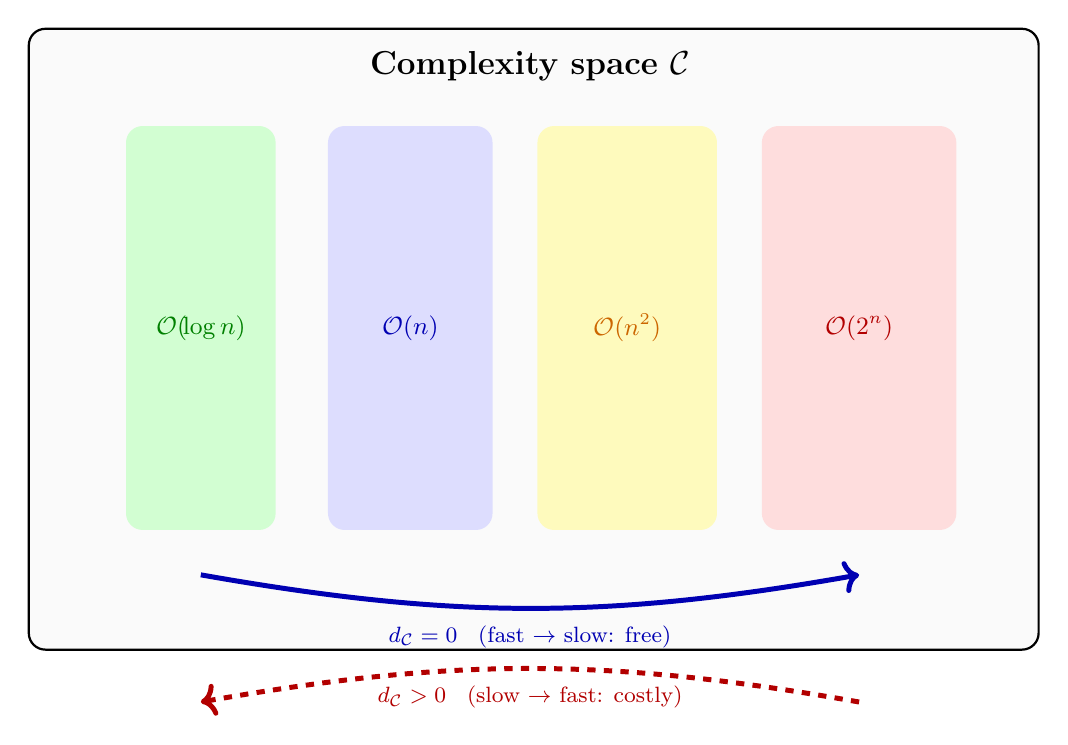
\begin{tikzpicture}[scale=0.95]
    \draw[thick, fill=gray!4, rounded corners=6pt] (-1.0,-4.3) rectangle (12.5,4.0);
    \node[font=\large\bfseries] at (5.7,3.5) {Complexity space $\C$};
    % Classes
    \fill[green!20, opacity=.85, rounded corners=6pt]
         (0.3,-2.7) rectangle (2.3,2.7);
    \node[font=\small, green!50!black, align=center] at (1.3,0) {$\BigO(\!\log n)$};
    \fill[blue!15, opacity=.85, rounded corners=6pt]
         (3.0,-2.7) rectangle (5.2,2.7);
    \node[font=\small, blue!70!black] at (4.1,0) {$\BigO(n)$};
    \fill[yellow!30, opacity=.85, rounded corners=6pt]
         (5.8,-2.7) rectangle (8.2,2.7);
    \node[font=\small, orange!80!black] at (7.0,0) {$\BigO(n^2)$};
    \fill[red!15, opacity=.85, rounded corners=6pt]
         (8.8,-2.7) rectangle (11.4,2.7);
    \node[font=\small, red!70!black] at (10.1,0) {$\BigO(2^n)$};
    % Arrows
    \draw[->, very thick, blue!70!black, line width=1.8pt]
         (1.3,-3.3) to[bend right=10]
         node[below=2pt, font=\footnotesize, pos=0.5] {$d_\C=0$ \;\;(fast $\to$ slow: free)}
         (10.1,-3.3);
    \draw[->, very thick, red!70!black, dashed, line width=1.8pt]
         (10.1,-5.0) to[bend right=10]
         node[below=2pt, font=\footnotesize, pos=0.5] {$d_\C>0$ \;\;(slow $\to$ fast: costly)}
         (1.3,-5.0);
\end{tikzpicture}
\caption{The complexity landscape.  Moving from a faster class to a
slower one is free ($d_\C=0$); the reverse direction is costly ($d_\C>0$).}
\label{fig:complexity-landscape}
\end{figure}


\subsection{Illustrative examples}

To build intuition, let us compute $d_\C$ for several pairs of
common complexity functions.

\begin{example}[Linear vs.\ quadratic]\label{ex:lin-quad}
Let $f(n)=n$ and $g(n)=n^2$.  Since $f(n)\le g(n)$ for all
$n\ge 1$, Theorem~\ref{thm:dc-props}(ii) gives $d_\C(f,g)=0$.
In the reverse direction,
\[
  d_\C(g,f)
  = \sum_{n=1}^{\infty}2^{-n}\max\!\left\{0,\frac{1}{n}-\frac{1}{n^2}\right\}
  = \sum_{n=2}^{\infty}2^{-n}\cdot\frac{n-1}{n^2},
\]
since the $n=1$ term vanishes ($\frac{1}{1}-\frac{1}{1}=0$).
We compute the first few partial sums to see how the series converges:
\begin{align*}
S_2 &= \tfrac{1}{4}\cdot\tfrac{1}{4} = 0.0625, \\
S_3 &= S_2 + \tfrac{1}{8}\cdot\tfrac{2}{9}
     = 0.0625 + 0.0278 = 0.0903, \\
S_4 &= S_3 + \tfrac{1}{16}\cdot\tfrac{3}{16}
     = 0.0903 + 0.0117 = 0.1020, \\
S_5 &= S_4 + \tfrac{1}{32}\cdot\tfrac{4}{25}
     = 0.1020 + 0.0050 = 0.1070.
\end{align*}
The series converges rapidly due to the $2^{-n}$ factor; by $n=10$
the partial sum is already $0.1108$, within $0.001$ of the limit.
Analytically, splitting $\frac{n-1}{n^2}=\frac{1}{n}-\frac{1}{n^2}$ and
using $\sum_{n=1}^\infty\frac{x^n}{n}=-\!\ln(1-x)$ and
$\sum_{n=1}^\infty\frac{x^n}{n^2}=\operatorname{Li}_2(x)$ at $x=\tfrac12$
gives the closed form
\[
  d_\C(g,f) = \ln 2 - \operatorname{Li}_2\!\bigl(\tfrac12\bigr)
  \approx 0.693 - 0.582 = 0.111.
\]
The exact value of the series can be confirmed symbolically
using SageMath; see
\href{\repourl/blob/main/code/sagemath/complexity_distances.sage}{\texttt{complexity\_distances.sage}}
in the companion repository.
The asymmetry is clear: moving from linear to quadratic is free, but
moving from quadratic to linear costs approximately~$0.111$.
\end{example}

\begin{example}[Logarithmic vs.\ linear]\label{ex:log-lin}
Let $f(n)=\ln(n+1)$ and $g(n)=n$.  Since $\ln(n+1)\le n$ for all
$n\ge 1$, we have $d_\C(f,g)=0$.  But $d_\C(g,f)>0$ because $g$
is slower.  The partial sums are:
\begin{align*}
S_1 &= \tfrac{1}{2}\bigl(\tfrac{1}{\ln 2}-1\bigr) \approx 0.2213, \quad
S_2 = S_1 + \tfrac{1}{4}\bigl(\tfrac{1}{\ln 3}-\tfrac{1}{2}\bigr) \approx 0.3179, \\
S_3 &\approx 0.3609, \quad
S_5 \approx 0.3991, \quad
S_{10} \approx 0.4165.
\end{align*}
The limit is $d_\C(g,f)\approx 0.417$; for exact symbolic evaluation see
\href{\repourl/blob/main/code/sagemath/complexity_distances.sage}{\texttt{complexity\_distances.sage}}.
\end{example}

\begin{example}[Equal functions]\label{ex:equal}
If $f=g$, then $d_\C(f,g)=d_\C(g,f)=0$.  The distance is
symmetric (and zero) for identical functions, as expected.
\end{example}

\begin{example}[Constant shift]\label{ex:constant-shift}
Let $f(n)=n$ and $g(n)=n+c$ for some constant $c>0$.  Then
$f(n)<g(n)$ for all~$n$, so $d_\C(f,g)=0$.  In the reverse
direction, $d_\C(g,f)=\sum_{n=1}^\infty 2^{-n}\cdot c/(n(n+c))$,
which is small but positive---reflecting the fact that~$g$ is only
slightly slower.
\end{example}


\begin{example}[Incomparable functions]\label{ex:incomparable}
Let $f(n)=n+(-1)^{n+1}$ and $g(n)=n$.  Then $f(1)=2>1=g(1)$ but
$f(2)=1<2=g(2)$, so neither $f(n)\le g(n)$ nor $g(n)\le f(n)$
for all~$n$.  (Note that $f$ alternates above and below~$g$: $f$
exceeds $g$ at odd indices and falls below at even indices.)
Consequently, \emph{both} $d_\C(f,g)>0$ and $d_\C(g,f)>0$.
Only odd-index terms contribute to $d_\C(f,g)$:
\[
  d_\C(f,g) = \sum_{\substack{n\ge 1\\n\text{ odd}}}
  \frac{2^{-n}}{n(n+1)}
  = \tfrac{1}{2}\cdot\tfrac{1}{2}
    +\tfrac{1}{8}\cdot\tfrac{1}{12}+\cdots
  \approx 0.262.
\]
Similarly, only even-index terms contribute to $d_\C(g,f)$:
\[
  d_\C(g,f) = \sum_{\substack{n\ge 2\\n\text{ even}}}
  \frac{2^{-n}}{n(n-1)}
  = \tfrac{1}{4}\cdot\tfrac{1}{2}
    +\tfrac{1}{16}\cdot\tfrac{1}{12}+\cdots
  \approx 0.131.
\]
The symmetrized distance is
$d_\C^s(f,g)=\max\{0.262,0.131\}\approx 0.262$.
Observe that $d_\C(f,g)\approx 2\,d_\C(g,f)$: the
``upward oscillation'' is costlier than the ``downward'' one,
reflecting the asymmetry of the quasi-metric.
The exact sums are verified symbolically in
\href{\repourl/blob/main/code/sagemath/incomparable_functions.sage}{\texttt{incomparable\_functions.sage}}.
\end{example}

\begin{example}[Counterexample: unbounded reciprocal difference]\label{ex:counter-bounded}
Let $f(n)=1/n$ (efficiency improves with $n$) and $g(n)=1$.  Then
$1/g(n)-1/f(n)=1-n$, which is negative for $n\ge 2$, so only
the $n=1$ term contributes: $d_\C(f,g)=2^{-1}\max\{0,1-1\}=0$.
In the reverse direction, $1/f(n)-1/g(n)=n-1$, so
$d_\C(g,f)=\sum_{n=2}^\infty 2^{-n}(n-1)=1$.  This example
saturates the upper bound of Theorem~\ref{thm:dc-props}(iii),
showing that $d_\C(f,g)\le 1$ is tight.
\end{example}

\subsection{The conjugate and symmetrized complexity distances}

Since $d_\C$ is a quasi-metric, we automatically obtain the conjugate
and symmetrization.

\begin{proposition}\label{prop:conjugate-dc}
The conjugate of the complexity quasi-metric is
\[
  d_\C^t(f,g) \;=\; d_\C(g,f)
  \;=\; \sum_{n=1}^{\infty}2^{-n}\max\!\left\{0,\frac{1}{f(n)}-\frac{1}{g(n)}\right\}.
\]
The symmetrization is $d_\C^s(f,g)=\max\{d_\C(f,g),d_\C(g,f)\}$.
\end{proposition}

\begin{proof}
By Definition~\ref{def:conjugate}, $d_\C^t(f,g)=d_\C(g,f)$.
Substituting $g$ for the first argument and $f$ for the second
in Definition~\ref{def:dc} yields the stated formula.  That
$d_\C^s=\max\{d_\C,d_\C^t\}$ is a metric follows from the
general theory (Definition~\ref{def:conjugate}).
\end{proof}

The symmetrized distance $d_\C^s$ is a genuine metric on $\C$ and
measures the ``worst-case directional cost'' between two complexity
functions.

\begin{example}[Symmetrization of linear vs.\ quadratic]\label{ex:sym}
From Example~\ref{ex:lin-quad}, $d_\C(f,g)=0$ and
$d_\C(g,f)\approx 0.111$, so $d_\C^s(f,g)\approx 0.111$.
\end{example}


\subsection{Computing the complexity quasi-metric}

We now describe an algorithm for numerically approximating $d_\C(f,g)$.
Since the series involves infinitely many terms, we truncate at
$N$~terms; the exponential decay of $2^{-n}$ ensures rapid convergence.

\begin{algorithm}[H]
\DontPrintSemicolon
\SetAlgoLined
\KwIn{Functions $f,g$; truncation parameter $N$}
\KwOut{Approximation of $d_\C(f,g)$}
$S \leftarrow 0$\;
\For{$n \leftarrow 1$ \KwTo $N$}{
    $\Delta \leftarrow 1/g(n) - 1/f(n)$\;
    \If{$\Delta > 0$}{
        $S \leftarrow S + 2^{-n}\,\Delta$\;
    }
}
\Return{$S$}\;
\caption{Compute $d_\C(f,g)$}
\label{alg:dc}
\end{algorithm}

\begin{remark}[Convergence rate]
The truncation error after $N$ terms is at most $2^{-N}$, since each
omitted term contributes at most $2^{-n}$.  In practice, $N=80$ gives
accuracy well beyond double-precision floating-point.
\end{remark}

A Python implementation of Algorithm~\ref{alg:dc} is provided in
\href{\repourl/blob/main/code/python/complexity_distance.py}{\texttt{complexity\_distance.py}}.
For many common function pairs, the infinite series admits a
closed-form evaluation via symbolic algebra; we use SageMath for
exact verification throughout (see
\href{\repourl/tree/main/code/sagemath}{\texttt{code/sagemath/}}).


% ═══════════════════════════════════════════════════════════════
\section{Expansive homeomorphisms}
\label{sec:expansive}
% ═══════════════════════════════════════════════════════════════

We now turn to the dynamical ingredient of our theory.
The notion of an expansive homeomorphism captures the idea that a
map ``spreads things out'': no two distinct points can remain close
forever under iteration.

\subsection{Definition and motivation}

In a standard metric space, expansiveness was introduced by
Utz~\cite{utz1950}: a homeomorphism $\psi\colon X\to X$ is
\emph{expansive} if there exists a constant $\delta>0$ such that for
every pair of distinct points $x\neq y$, some iterate $\psi^n$
separates them by more than~$\delta$.  The constant~$\delta$ is
called the \emph{expansive constant}.

Olela Otafudu et al.~\cite{olela2024} extended this to
quasi-metric spaces, where the asymmetry of the distance introduces
new subtleties.

\begin{definition}[Expansive homeomorphism~\cite{olela2024}]
\label{def:expansive}
Let $(X,q)$ be a quasi-metric space and let $\psi\colon X\to X$ be a
homeomorphism (with respect to the topology $\tau_{q^s}$ induced by
the symmetrization).  We say $\psi$ is \emph{$q$-expansive} if there
exists $\delta>0$ such that for all $x\neq y$, there exists $n\in\Z$
with $q(\psi^n(x),\psi^n(y))>\delta$.
\end{definition}

Note that we allow both positive and negative iterates: the
separation may occur in the future or in the past.  This is essential
in the quasi-metric setting, because the asymmetry of $q$ means that
forward and backward iterates may behave very differently.

\begin{figure}[H]
\centering
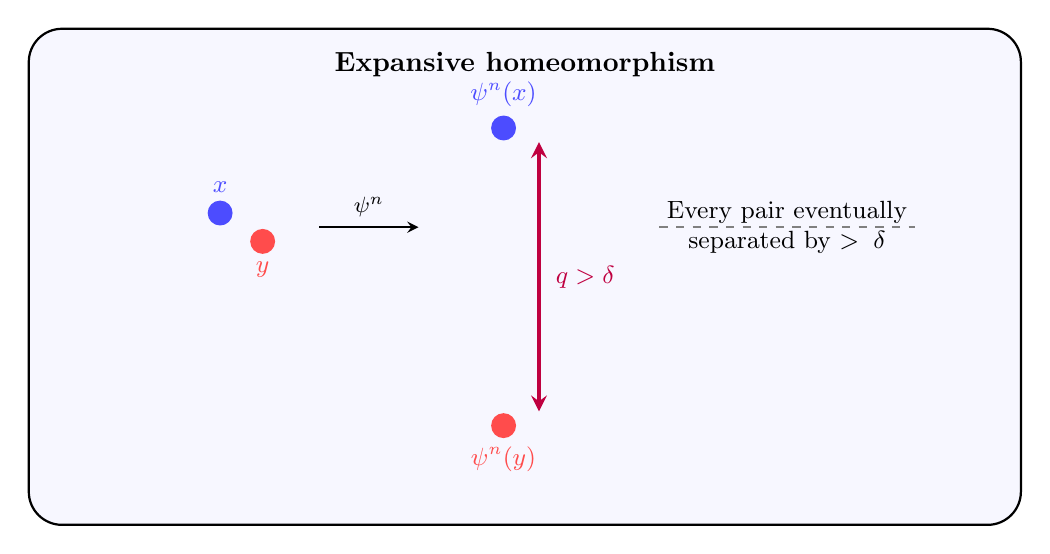
\begin{tikzpicture}[scale=0.9, >=stealth]
  % Box
  \draw[thick, fill=blue!3, rounded corners=12pt] (-1.5,-3.0) rectangle (12.5,4.0);
  \node[font=\bfseries] at (5.5,3.5) {Expansive homeomorphism};
  % Two points
  \fill[blue!70] (1.2,1.4) circle (5pt) node[above=4pt, font=\small] {$x$};
  \fill[red!70]  (1.8,1.0) circle (5pt) node[below=4pt, font=\small] {$y$};
  % Arrow
  \draw[thick, ->] (2.6,1.2) -- (4.0,1.2) node[midway, above, font=\footnotesize] {$\psi^n$};
  % Separated points
  \fill[blue!70] (5.2,2.6) circle (5pt) node[above=4pt, font=\small] {$\psi^n(x)$};
  \fill[red!70]  (5.2,-1.6) circle (5pt) node[below=4pt, font=\small] {$\psi^n(y)$};
  % Distance
  \draw[<->, thick, purple, line width=1.5pt] (5.7,2.4) -- (5.7,-1.4);
  \node[right, purple, font=\small] at (5.8,0.5) {$q > \delta$};
  % Note
  \draw[thick, dashed, gray] (7.4,1.2) -- (11.0,1.2);
  \node[font=\small, text width=3.8cm, align=center] at (9.2,1.2)
    {Every pair eventually separated by $>\delta$};
\end{tikzpicture}
\caption{An expansive homeomorphism: the orbits of any two distinct
points are eventually separated by more than~$\delta$.}
\label{fig:expansive-idea}
\end{figure}


\subsection{Equivalences in the quasi-metric setting}

A key result of~\cite{olela2024} is that expansiveness with respect
to~$q$ is equivalent to expansiveness with respect to the conjugate~$q^t$.

\begin{theorem}[\cite{olela2024}]\label{thm:olela-equiv}
Let $(X,q)$ be a quasi-metric space and $\psi\colon X\to X$ a
homeomorphism.  Then:
\begin{enumerate}[label=\textup{(\roman*)}]
  \item $\psi$ is $q$-expansive if and only if $\psi$ is $q^t$-expansive.
  \item If $\psi$ is $q$-expansive, then $\psi$ is $q^s$-expansive.
    The converse is false in general.
\end{enumerate}
\end{theorem}

Part~(i) is remarkable: it says that the direction of asymmetry does
not matter for the \emph{existence} of expansive behaviour, although
it may affect the value of the expansive constant.  Part~(ii) says
that quasi-metric expansiveness is a strictly stronger property than
metric expansiveness.

\begin{example}[Non-equivalence of (ii)]
\label{ex:converse-false}
Consider $X=\{0,1\}^\Z$ (the full two-shift) with the quasi-metric
$q(x,y)=\sum_{n\ge 0}2^{-n}|x_n-y_n|$ (only non-negative indices).
The shift map is $q^s$-expansive but not $q$-expansive, because
forward-only distances cannot detect differences in the past.
\end{example}

\begin{example}[Illustrating part~(i): $q$-expansive $\Leftrightarrow$ $q^t$-expansive]
\label{ex:q-qt-equiv}
Consider $f(n)=n$ and $g(n)=2n$ on $(\C,d_\C)$ with $\psi_2$.
We have $d_\C(f,g)=0$ (since $n\le 2n$) and
$d_\C(g,f)=\sum_{n=1}^\infty 2^{-n}\cdot\frac{1}{2n}
=\frac{1}{2}\sum_{n=1}^\infty\frac{(1/2)^n}{n}=\frac{1}{2}\ln 2
\approx 0.347$
(partial sums: $S_1=0.250$, $S_2=0.313$, $S_3=0.333$,
$S_5=0.344$; exact value: $\frac{1}{2}\ln 2$).
The backward iterates give $d_\C(\psi_2^{-k}(g),\psi_2^{-k}(f))
=2^k\cdot 0.347$, which exceeds any $\delta$ for $k$ large enough.
Thus $\psi_2$ is $d_\C$-expansive.  For the conjugate:
$d_\C^t(f,g)=d_\C(g,f)\approx 0.347>0$, and
$d_\C^t(\psi_2^{-k}(f),\psi_2^{-k}(g))=2^k\cdot 0.347\to\infty$.
So $\psi_2$ is also $d_\C^t$-expansive, confirming part~(i) of
Theorem~\ref{thm:olela-equiv}.
\end{example}

\begin{example}[Non-expansive homeomorphism: translation]
\label{ex:non-exp-translation}
Define the \emph{additive translation} $\phi_c(f)(n)=f(n)+c$ for a
fixed constant $c>0$.  Since $\phi_c^k(f)(n)=f(n)+kc$, we compute:
\[
  d_\C(\phi_c^k(f),\phi_c^k(g))
  = \sum_{n=1}^\infty 2^{-n}
    \max\!\left\{0,\frac{1}{g(n)+kc}-\frac{1}{f(n)+kc}\right\}.
\]
For large $|k|$, the terms $1/(f(n)+kc)$ and $1/(g(n)+kc)$ both
tend to zero (if $k\to+\infty$) or become undefined (if $kc$ is
large and negative).  In particular, for $k\to+\infty$,
$d_\C(\phi_c^k(f),\phi_c^k(g))\to 0$ for \emph{all} pairs $f,g$.
Since there is no $\delta>0$ that is eventually exceeded, $\phi_c$
is \emph{not} expansive.  Unlike the scaling map, additive
translation does not preserve the multiplicative structure needed
for expansiveness on~$(\C,d_\C)$.
\end{example}

\subsection{Checking expansiveness numerically}

Given two functions $f,g$ and a candidate map $\psi$, we can
numerically check whether their orbits separate.  The idea is simple:
iterate $\psi$ both forward and backward and check whether the
distance exceeds~$\delta$ at some iterate.

\begin{algorithm}[H]
\DontPrintSemicolon
\SetAlgoLined
\KwIn{Functions $f\neq g$; map $\psi$; candidate $\delta$;
      iteration bound $M$}
\KwOut{\texttt{True} if separation $>\delta$ found; the iterate $n$}
\For{$n \leftarrow -M$ \KwTo $M$}{
    $d \leftarrow q(\psi^n(f),\,\psi^n(g))$\;
    \If{$d > \delta$}{
        \Return{\texttt{True}, $n$}\;
    }
}
\Return{\texttt{False}, \texttt{None}}\;
\caption{Check expansive separation}
\label{alg:check-exp}
\end{algorithm}

A Python implementation is given in
\href{\repourl/blob/main/code/python/expansiveness_check.py}{\texttt{expansiveness\_check.py}}.


% ═══════════════════════════════════════════════════════════════
\section{The scaling transformation}
\label{sec:scaling}
% ═══════════════════════════════════════════════════════════════

We now introduce the main dynamical actor: the \emph{scaling
transformation} on the complexity space.  This is the simplest
non-trivial transformation that respects the multiplicative structure
of running-time functions.

\subsection{Definition and basic properties}

\begin{definition}[Scaling transformation]\label{def:scaling}
For $\alpha>0$, the \emph{scaling transformation}
$\psi_\alpha\colon\C\to\C$ is defined by
\[
  \psi_\alpha(f)(n) \;=\; \alpha\cdot f(n).
\]
Its $k$-th iterate is $\psi_\alpha^k(f)(n)=\alpha^k f(n)$.
\end{definition}

The map $\psi_\alpha$ multiplies every running-time value by the
constant~$\alpha$.  When $\alpha>1$, this makes algorithms
``slower'' (larger running times); when $0<\alpha<1$, it makes them
``faster.''  When $\alpha=1$, it is the identity.

\begin{example}[Scaling a linear function]
If $f(n)=n$ and $\alpha=2$, then $\psi_2(f)(n)=2n$,
$\psi_2^2(f)(n)=4n$, $\psi_2^3(f)(n)=8n$, and in general
$\psi_2^k(f)(n)=2^k n$.  The orbit of~$f$ under $\psi_2$
consists of all functions of the form $2^k n$ for $k\in\Z$.
\end{example}

\begin{example}[Scaling a quadratic function]
If $g(n)=n^2$ and $\alpha=3$, then $\psi_3^k(g)(n)=3^k n^2$.
The orbit consists of functions $3^k n^2$, which are all
quadratic but with different leading coefficients.
\end{example}

The key algebraic property of $\psi_\alpha$ with respect to $d_\C$
is that it acts as a \emph{Lipschitz contraction} (when $\alpha>1$)
or \emph{expansion} (when $\alpha<1$).

\begin{lemma}\label{lem:scaling-lip}
For any $\alpha>0$ and any $f,g\in\C$,
\[
  d_\C(\psi_\alpha(f),\psi_\alpha(g))
  \;=\; \frac{1}{\alpha}\,d_\C(f,g).
\]
\end{lemma}

\begin{proof}
We compute directly:
\begin{align*}
  d_\C(\psi_\alpha(f),\psi_\alpha(g))
  &= \sum_{n=1}^{\infty}2^{-n}\max\!\left\{0,
     \frac{1}{\alpha g(n)}-\frac{1}{\alpha f(n)}\right\}\\
  &= \sum_{n=1}^{\infty}2^{-n}\cdot\frac{1}{\alpha}\,
     \max\!\left\{0,\frac{1}{g(n)}-\frac{1}{f(n)}\right\}
  \;=\;\frac{1}{\alpha}\,d_\C(f,g). \qedhere
\end{align*}
\end{proof}

By induction, $d_\C(\psi_\alpha^k(f),\psi_\alpha^k(g))
=\alpha^{-k}\,d_\C(f,g)$ for all $k\ge 0$.

\begin{example}[Numerical verification of Lemma~\ref{lem:scaling-lip}]
\label{ex:lip-numerical}
Let $f(n)=n$, $g(n)=n^2$, and $\alpha=3$.  We have
$d_\C(g,f)\approx 0.111$.  After scaling:
$\psi_3(f)(n)=3n$ and $\psi_3(g)(n)=3n^2$.  Then
$d_\C(\psi_3(g),\psi_3(f))=d_\C(3n^2,3n)
=\sum_{n=1}^\infty 2^{-n}\max\!\left\{0,\frac{1}{3n}-\frac{1}{3n^2}\right\}
=\frac{1}{3}\cdot d_\C(g,f)\approx 0.037$, which matches
$\frac{1}{\alpha}\cdot 0.111=0.037$ exactly
as confirmed by SageMath
(\href{\repourl/blob/main/code/sagemath/partial_sums.sage}{\texttt{partial\_sums.sage}}).
\end{example}

\begin{remark}[Group structure]
The scaling maps form a multiplicative group:
$\psi_\alpha\circ\psi_\beta=\psi_{\alpha\beta}$ and
$\psi_\alpha^{-1}=\psi_{1/\alpha}$.  In particular, the family
$\{\psi_\alpha:\alpha>0\}$ is isomorphic to $(\R_{>0},\cdot)$.
The Lipschitz property of Lemma~\ref{lem:scaling-lip} extends
to this group action:
$d_\C(\psi_\alpha\circ\psi_\beta(f),\psi_\alpha\circ\psi_\beta(g))
=\frac{1}{\alpha\beta}\,d_\C(f,g)$.
\end{remark}

\begin{remark}[Interpretation]
When $\alpha>1$, forward iterates of $\psi_\alpha$ bring functions
\emph{closer} in the $d_\C$ distance (contraction by factor
$1/\alpha$ per step).  Backward iterates push them \emph{apart}
(expansion by factor $\alpha$ per step).  When $0<\alpha<1$, the
roles reverse.
\end{remark}


\subsection{Main theorem: Expansiveness of scaling}

We are now ready to state and prove our main result.  The theorem
asserts that the scaling map is expansive precisely when it is
non-trivial.

\begin{theorem}[Main theorem]\label{thm:main-scaling}
The scaling transformation $\psi_\alpha$ is expansive on $(\C,d_\C)$
if and only if $\alpha\neq 1$.
\end{theorem}

\begin{proof}
We consider three cases.

\textbf{Case 1: $\alpha=1$.}  The map $\psi_1$ is the identity, so
$d_\C(\psi_1^n(f),\psi_1^n(g))=d_\C(f,g)$ for all~$n$.  If
$d_\C(f,g)>0$, the distance is constant and may be smaller than any
proposed~$\delta$; if $d_\C(f,g)=0$ but $d_\C(g,f)>0$ (i.e., $f$ is
faster than~$g$), then $d_\C(\psi_1^n(f),\psi_1^n(g))=0$ for all~$n$
and no separation occurs.  Hence $\psi_1$ is not expansive.

\textbf{Case 2: $\alpha>1$.}  Let $f\neq g$.  By $T_0$~separation,
at least one of $d_\C(f,g)$ or $d_\C(g,f)$ is positive.  Suppose
$d_\C(f,g)>0$.  Then for negative iterates:
\[
  d_\C(\psi_\alpha^{-k}(f),\psi_\alpha^{-k}(g))
  \;=\; \alpha^k\,d_\C(f,g)
  \;\xrightarrow{k\to\infty}\;\infty.
\]
In particular, for any $\delta>0$ there exists $k$ with
$d_\C(\psi_\alpha^{-k}(f),\psi_\alpha^{-k}(g))>\delta$.

If instead $d_\C(f,g)=0$ but $d_\C(g,f)>0$, then by
Theorem~\ref{thm:olela-equiv}(i), $\psi_\alpha$ is also
$d_\C^t$-expansive, and we apply the same argument with $d_\C^t$.

\textbf{Case 3: $0<\alpha<1$.}  Now forward iterates expand:
\[
  d_\C(\psi_\alpha^k(f),\psi_\alpha^k(g))
  \;=\;\alpha^{-k}\,d_\C(f,g)
  \;\xrightarrow{k\to\infty}\;\infty.
\]
The argument is otherwise identical.
\end{proof}

\begin{example}[Expansiveness for $\alpha=2$]\label{ex:expansive-alpha2}
Consider $f(n)=n$ and $g(n)=n+1$. For $\alpha=2$, we have $d_\C(f,g)=0$
(since $f(n)<g(n)$ for all $n$) but
\[
  d_\C(g,f)=\sum_{n=1}^\infty
  \frac{2^{-n}}{n(n+1)}.
\]
Computing partial sums: $S_1=\frac{1}{4}=0.250$,
$S_2=S_1+\frac{1}{24}\approx 0.292$,
$S_3\approx 0.302$, $S_5\approx 0.306$, converging to
$\approx 0.307$
(see \href{\repourl/blob/main/code/sagemath/complexity_distances.sage}{\texttt{complexity\_distances.sage}}).
The backward iterates give:
\[
d_\C(\psi_2^{-k}(g),\psi_2^{-k}(f)) = 2^k \cdot 0.307
\]
For $\delta=0.5$, we need $2^k \cdot 0.307 > 0.5$, i.e., $k \geq 1$.
Indeed, $d_\C(\psi_2^{-1}(g),\psi_2^{-1}(f)) \approx 0.614 > 0.5$.
Thus $\psi_2$ is expansive with expansive constant $\delta=0.5$.
\end{example}

\begin{example}[Non-expansiveness for $\alpha=1$]\label{ex:non-expansive-alpha1}
Take $f(n)=n$ and $g(n)=n^2$. For $\alpha=1$, $\psi_1$ is the identity, 
so $d_\C(\psi_1^n(f),\psi_1^n(g)) = d_\C(f,g)=0$ for all $n$, 
while $d_\C(\psi_1^n(g),\psi_1^n(f)) = d_\C(g,f)\approx 0.111$ for all $n$.
No matter how large $n$ is, $d_\C(f,g)$ remains $0$, so no separation occurs 
in that direction. Therefore $\psi_1$ is not expansive.
\end{example}

\begin{figure}[H]
\centering
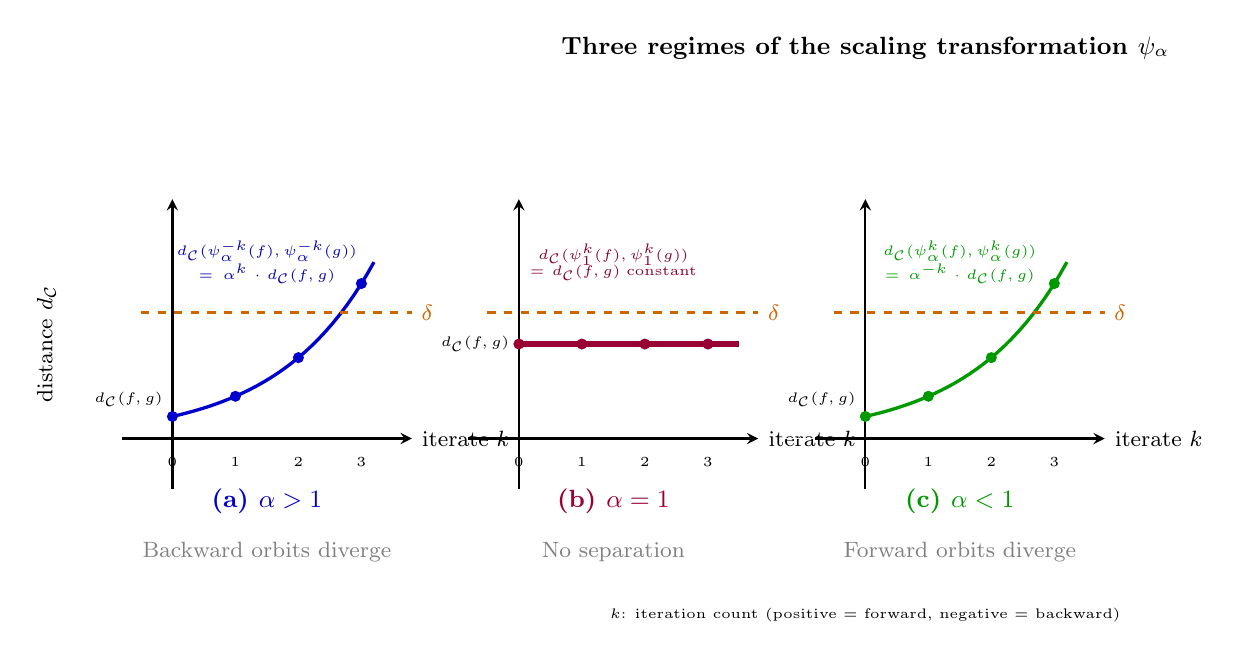
\begin{tikzpicture}[scale=0.8]
    % Title with more space above
    \node[font=\small\bfseries] at (5.5,6.2) {Three regimes of the scaling transformation $\psi_\alpha$};
    
    % Case alpha > 1 - with shorter axes
    \begin{scope}[shift={(-5.5,0)}]
        \draw[thick, ->, >=stealth] (-0.8,0) -- (3.8,0) node[right, font=\footnotesize] {iterate $k$};
        \draw[thick, ->, >=stealth] (0,-0.8) -- (0,3.8);
        \node[font=\small\bfseries, blue!80!black] at (1.5,-1.0) {(a) $\alpha > 1$};
        
        % Exponential growth curve (backward iterates) - shorter domain
        \draw[very thick, blue!80!black, domain=0:3.2, samples=30]
             plot (\x, {0.35*exp(0.65*\x)});
        
        % Delta threshold line - positioned appropriately
        \draw[thick, orange!80!black, dashed] (-0.5,2.0) -- (3.8,2.0);
        \node[orange!80!black, right, font=\footnotesize] at (3.8,2.0) {$\delta$};
        
        % Annotations - moved closer to curve
        \node[font=\tiny, align=center, text width=2.5cm, blue!70!black] at (1.5,2.8) 
             {$d_\C(\psi_\alpha^{-k}(f),\psi_\alpha^{-k}(g))$\\$=\alpha^k \cdot d_\C(f,g)$};
        
        \node[font=\footnotesize, gray, align=center] at (1.5,-1.8) 
             {Backward orbits diverge};
             
        % Example points - fewer points
        \foreach \k in {0,1,2,3} {
            \fill[blue!80!black] (\k, {0.35*exp(0.65*\k)}) circle (2.5pt);
        }
        
        % Iterate labels
        \foreach \k in {0,1,2,3} {
            \node[font=\tiny, below] at (\k,-0.15) {$\k$};
        }
        
        \node[font=\tiny, above left] at (0,0.35) {$d_\C(f,g)$};
    \end{scope}
    
    % Vertical space between cases
    \draw[white] (4.2,0) -- (4.8,0); % Invisible spacer
    
    % Case alpha = 1 - with shorter axes
    \begin{scope}[shift={(0,0)}]
        \draw[thick, ->, >=stealth] (-0.8,0) -- (3.8,0) node[right, font=\footnotesize] {iterate $k$};
        \draw[thick, ->, >=stealth] (0,-0.8) -- (0,3.8);
        \node[font=\small\bfseries, purple!80!black] at (1.5,-1.0) {(b) $\alpha = 1$};
        
        % Constant line (identity map) - shorter
        \draw[very thick, purple!80!black, line width=2.2pt] (0,1.5) -- (3.5,1.5);
        
        % Delta threshold line
        \draw[thick, orange!80!black, dashed] (-0.5,2.0) -- (3.8,2.0);
        \node[orange!80!black, right, font=\footnotesize] at (3.8,2.0) {$\delta$};
        
        % Annotations
        \node[font=\tiny, align=center, text width=2.5cm, purple!70!black] at (1.5,2.8) 
             {$d_\C(\psi_1^k(f),\psi_1^k(g))$\\$= d_\C(f,g)$ constant};
        
        \node[font=\footnotesize, gray, align=center] at (1.5,-1.8) 
             {No separation};
             
        % Iterate labels
        \foreach \k in {0,1,2,3} {
            \node[font=\tiny, below] at (\k,-0.15) {$\k$};
            \fill[purple!80!black] (\k,1.5) circle (2.5pt);
        }
        
        \node[font=\tiny, left] at (0,1.5) {$d_\C(f,g)$};
    \end{scope}
    
    % Vertical space between cases
    \draw[white] (4.2,0) -- (4.8,0); % Invisible spacer
    
    % Case alpha < 1 - with shorter axes
    \begin{scope}[shift={(5.5,0)}]
        \draw[thick, ->, >=stealth] (-0.8,0) -- (3.8,0) node[right, font=\footnotesize] {iterate $k$};
        \draw[thick, ->, >=stealth] (0,-0.8) -- (0,3.8);
        \node[font=\small\bfseries, green!60!black] at (1.5,-1.0) {(c) $\alpha < 1$};
        
        % Exponential growth curve (forward iterates) - shorter domain
        \draw[very thick, green!60!black, domain=0:3.2, samples=30]
             plot (\x, {0.35*exp(0.65*\x)});
        
        % Delta threshold line
        \draw[thick, orange!80!black, dashed] (-0.5,2.0) -- (3.8,2.0);
        \node[orange!80!black, right, font=\footnotesize] at (3.8,2.0) {$\delta$};
        
        % Annotations
        \node[font=\tiny, align=center, text width=2.5cm, green!60!black] at (1.5,2.8) 
             {$d_\C(\psi_\alpha^k(f),\psi_\alpha^k(g))$\\$=\alpha^{-k} \cdot d_\C(f,g)$};
        
        \node[font=\footnotesize, gray, align=center] at (1.5,-1.8) 
             {Forward orbits diverge};
             
        % Example points
        \foreach \k in {0,1,2,3} {
            \fill[green!60!black] (\k, {0.35*exp(0.65*\k)}) circle (2.5pt);
        }
        
        % Iterate labels
        \foreach \k in {0,1,2,3} {
            \node[font=\tiny, below] at (\k,-0.15) {$\k$};
        }
        
        \node[font=\tiny, above left] at (0,0.35) {$d_\C(f,g)$};
    \end{scope}
    
    % Common y-axis label
    \node[font=\footnotesize, rotate=90] at (-7.5,1.5) {distance $d_\C$};
    
    % Common x-axis explanation
    \node[font=\tiny, align=center] at (5.5,-2.8) 
         {$k$: iteration count (positive = forward, negative = backward)};
\end{tikzpicture}
\vspace{0.2cm}
\caption{The three regimes of the scaling transformation $\psi_\alpha$. 
(a) For $\alpha>1$, backward iterates cause exponential separation: 
$d_\C(\psi_\alpha^{-k}(f),\psi_\alpha^{-k}(g)) = \alpha^k d_\C(f,g)$. 
(b) For $\alpha=1$, the map is the identity and distances remain constant. 
(c) For $0<\alpha<1$, forward iterates cause exponential separation: 
$d_\C(\psi_\alpha^k(f),\psi_\alpha^k(g)) = \alpha^{-k} d_\C(f,g)$. 
In cases (a) and (c), for any $\delta>0$, there exists $k$ such that the 
distance exceeds $\delta$, making $\psi_\alpha$ expansive.}
\label{fig:three-cases}
\end{figure}

\begin{example}[Concrete separation for $\alpha=2$]\label{ex:concrete-sep}
Let $f(n)=n$, $g(n)=n+1$, and $\alpha=2$.  Then $d_\C(f,g)=0$
(since $f(n)<g(n)$) and $d_\C(g,f)>0$.  After $k$~backward
iterates, $d_\C(\psi_2^{-k}(g),\psi_2^{-k}(f))=2^k\,d_\C(g,f)$.
Even with $d_\C(g,f)$ small, a few backward steps suffice to
exceed any given~$\delta$.  A numerical verification is given in
\href{\repourl/blob/main/code/python/expansiveness_check.py}{\texttt{expansiveness\_check.py}}.
\end{example}

\begin{example}[Separation for $\alpha=1/3$]\label{ex:sep-third}
Let $f(n)=n^2$, $g(n)=n^3$, and $\alpha=1/3$.  Here
$d_\C(f,g)=0$ but $d_\C(g,f)>0$.  After $k$~forward iterates,
$d_\C(\psi_{1/3}^k(g),\psi_{1/3}^k(f))=3^k\,d_\C(g,f)\to\infty$.
\end{example}


\subsection{The expansive constant}

For a given $\alpha\neq 1$ and pair $f\neq g$, one may ask: what is
the \emph{smallest} iterate~$n$ at which separation occurs?  This
depends on the initial distance and the value of~$\alpha$.

\begin{proposition}[Separation iterate]\label{prop:sep-iterate}
Let $\alpha>1$ and let $f,g\in\C$ with $d:=d_\C(f,g)>0$.  Then
$d_\C(\psi_\alpha^{-k}(f),\psi_\alpha^{-k}(g))>\delta$ for all
$k\ge\lceil\log_\alpha(\delta/d)\rceil$.
\end{proposition}

\begin{proof}
We need $\alpha^k d>\delta$, i.e.,
$k>\log_\alpha(\delta/d)$.
\end{proof}

\begin{example}[Computing the separation iterate]\label{ex:sep-iterate-num}
Let $\alpha=2$, $f(n)=n^2$, $g(n)=n$, and $\delta=0.5$.  Since
$f(n)\ge g(n)$ for $n\ge 1$, we have $d:=d_\C(f,g)>0$.
Numerically, $d\approx 0.111$.  By Proposition~\ref{prop:sep-iterate},
separation occurs for
$k\ge\lceil\log_2(0.5/0.111)\rceil=\lceil\log_2(4.50)\rceil
=\lceil 2.17\rceil=3$.
Indeed, $d_\C(\psi_2^{-3}(f),\psi_2^{-3}(g))=8\cdot 0.111
=0.888>0.5$.  For $k=2$: $4\cdot 0.111=0.444<0.5$, confirming
that $k=3$ is the \emph{first} iterate achieving separation
(verified in
\href{\repourl/blob/main/code/sagemath/separation_iterates.sage}{\texttt{separation\_iterates.sage}}).
\end{example}

\begin{example}[Counterexample: $\alpha$ close to 1 delays separation]\label{ex:slow-sep}
Let $\alpha=1.01$, $f(n)=n$, $g(n)=n+1$, and $\delta=0.5$.
Then $d:=d_\C(g,f)\approx 0.307$.  The separation iterate satisfies
$k\ge\lceil\log_{1.01}(0.5/0.307)\rceil=\lceil\log_{1.01}(1.63)\rceil
\approx\lceil 49.1\rceil=50$.
Thus $\alpha$ close to~$1$ requires $50$ backward iterates
for separation, while $\alpha=2$ needs only~$3$ (Example~\ref{ex:sep-iterate-num}).
This illustrates that the ``speed'' of expansiveness is controlled
by $\log\alpha$
(see \href{\repourl/blob/main/code/sagemath/separation_iterates.sage}{\texttt{separation\_iterates.sage}}).
\end{example}


% ═══════════════════════════════════════════════════════════════
\section{Stable and unstable sets}
\label{sec:stable-unstable}
% ═══════════════════════════════════════════════════════════════

The theory of expansive homeomorphisms naturally leads to the study
of \emph{stable} and \emph{unstable sets}: the collections of
points whose orbits remain close to a given orbit in forward or
backward time, respectively.  In our setting, these sets will turn
out to have a beautiful interpretation in terms of complexity classes.

\subsection{Stable sets}

\begin{definition}[Stable set]\label{def:stable}
Let $(X,q)$ be a quasi-metric space and $\psi\colon X\to X$ a
homeomorphism.  The \emph{$\delta$-stable set} of $f\in X$ is
\[
  S_q(f,\delta,\psi)
  \;=\; \{g\in X : q(\psi^n(f),\psi^n(g))\le\delta
    \text{ for all }n\ge 0\}.
\]
\end{definition}

For the scaling transformation on the complexity space, the stable
sets have a particularly clean description.

\begin{theorem}[Stable sets = complexity classes]\label{thm:stable-sets}
For $\alpha>1$, the $\delta$-stable set of $f$ under $\psi_\alpha$
in the complexity quasi-metric is
\[
  S_{d_\C}(f,\delta,\psi_\alpha)
  \;=\; \{g\in\C : d_\C(f,g)\le\delta\}.
\]
In particular, this set contains all $g$ with $g(n)\ge f(n)$ for
every~$n$---that is, all functions that are ``at least as slow
as~$f$.''
\end{theorem}

\begin{proof}
For $n\ge 0$, $d_\C(\psi_\alpha^n(f),\psi_\alpha^n(g))
=\alpha^{-n}d_\C(f,g)$.  Since $\alpha>1$, this is a decreasing
sequence, maximized at $n=0$ where it equals $d_\C(f,g)$.
Therefore
\[
  g\in S_{d_\C}(f,\delta,\psi_\alpha)
  \;\Longleftrightarrow\;
  \sup_{n\ge 0}\alpha^{-n}d_\C(f,g)\le\delta
  \;\Longleftrightarrow\;
  d_\C(f,g)\le\delta.
\]
If $g(n)\ge f(n)$ for all~$n$, then $d_\C(f,g)=0\le\delta$, so
$g$ is in the stable set.
\end{proof}

\begin{example}[Stable set of $f(n)=n$]\label{ex:stable-lin}
Take $f(n)=n$, $\alpha=2$, $\delta=0.1$. The stable set includes:
\begin{itemize}
\item $g_1(n)=n^2$ ($d_\C(f,g_1)=0\le 0.1$)
\item $g_2(n)=2n$ ($d_\C(f,g_2)=0\le 0.1$)
\item $g_3(n)=n+10$ ($d_\C(f,g_3)=0\le 0.1$)
\item $g_4(n)=n\sqrt{n}$ ($d_\C(f,g_4)=0\le 0.1$, since $n\le n\sqrt{n}$)
\end{itemize}
However, $h(n)=\sqrt{n}$ is NOT in the stable set because
$d_\C(f,h)\approx 0.113 > 0.1$.
\end{example}

\begin{example}[Counterexample: stability depends on $\delta$]\label{ex:counter-stable}
For $f(n)=n$, $g(n)=\sqrt{n}$, and $\alpha=2$, we have
$d_\C(f,g)=\sum_{n=2}^\infty 2^{-n}\bigl(\frac{1}{\sqrt{n}}-\frac{1}{n}\bigr)
\approx 0.113$ (since $\sqrt{n}<n$ for $n\ge 2$).
\begin{itemize}
\item If $\delta=0.2$, then $g\in S_{d_\C}(f,0.2,\psi_2)$ since $d_\C(f,g)\approx 0.113 < 0.2$.
\item If $\delta=0.05$, then $g\notin S_{d_\C}(f,0.05,\psi_2)$ since $d_\C(f,g)\approx 0.113 > 0.05$.
\end{itemize}
This shows the $\delta$-stable set shrinks as $\delta$ decreases
(see \href{\repourl/blob/main/code/sagemath/separation_iterates.sage}{\texttt{separation\_iterates.sage}}
for verification).
\end{example}

\begin{insightbox}[Complexity-theoretic interpretation]
The stable set $S_{d_\C}(f,\delta,\psi_\alpha)$ is the
``neighbourhood of slower functions around~$f$.''  In complexity
theory terms, it is a kind of asymptotic complexity class: it
contains all functions whose running time is ``close to or worse
than'' that of~$f$, where closeness is measured by $d_\C$.
\end{insightbox}


\subsection{Unstable sets}

\begin{definition}[Unstable set]\label{def:unstable}
The \emph{$\delta$-unstable set} of $f$ is
\[
  U_q(f,\delta,\psi)
  \;=\; \{g\in X : q(\psi^{-n}(f),\psi^{-n}(g))\le\delta
    \text{ for all }n\ge 0\}.
\]
\end{definition}

\begin{theorem}[Unstable sets]\label{thm:unstable-sets}
For $\alpha>1$, the $\delta$-unstable set of $f$ under $\psi_\alpha$
with respect to the \emph{conjugate} quasi-metric $d_\C^t$ is
\[
  U_{d_\C^t}(f,\delta,\psi_\alpha)
  \;=\; \{g\in\C : d_\C(g,f)=0\}.
\]
In particular, this set is independent of~$\delta$ and equals the set
of all $g$ with $g(n)\le f(n)$ for every~$n$---that is,
all functions that are ``at least as fast as~$f$.''
\end{theorem}

\begin{proof}
By definition,
$g\in U_{d_\C^t}(f,\delta,\psi_\alpha)$ iff
$d_\C^t(\psi_\alpha^{-n}(f),\psi_\alpha^{-n}(g))\le\delta$
for all $n\ge 0$.  Since
$d_\C^t(h_1,h_2)=d_\C(h_2,h_1)$, this becomes
$d_\C(\psi_\alpha^{-n}(g),\psi_\alpha^{-n}(f))\le\delta$ for all
$n\ge 0$.  By Lemma~\ref{lem:scaling-lip},
\[
  d_\C(\psi_\alpha^{-n}(g),\psi_\alpha^{-n}(f))
  \;=\;\alpha^n\,d_\C(g,f).
\]
Since $\alpha>1$, this is an increasing sequence.  If
$d_\C(g,f)>0$, then $\alpha^n d_\C(g,f)\to\infty$, which
eventually exceeds~$\delta$.  Hence $g$ is in the unstable set if and
only if $d_\C(g,f)=0$.

By Theorem~\ref{thm:dc-props}(ii), $d_\C(g,f)=0$ if and only if
$g(n)\le f(n)$ for all~$n$, so the unstable set consists precisely
of the functions that are pointwise at most~$f$.
\end{proof}

\begin{example}[Unstable set of $f(n)=n^2$]\label{ex:unstable-quad}
Take $f(n)=n^2$, $\alpha=2$, $\delta=0.1$. By Theorem~\ref{thm:unstable-sets},
the unstable set consists of all $g$ with $d_\C(g,f)=0$, i.e., $g(n)\le f(n)=n^2$
for all~$n$.  It includes:
\begin{itemize}
\item $g_1(n)=n$ ($n\le n^2$ for all $n\ge 1$, so $d_\C(g_1,f)=0$)
\item $g_2(n)=n\log(n+1)$ ($n\log(n+1)\le n^2$ for all $n\ge 1$, so $d_\C(g_2,f)=0$)
\item $g_3(n)=n^{1.5}$ ($n^{1.5}\le n^2$ for all $n\ge 1$, so $d_\C(g_3,f)=0$)
\end{itemize}
But $h(n)=2^n$ is NOT in the unstable set because $2^n>n^2$ for
large~$n$, so $d_\C(h,f)>0$.
\end{example}

\begin{insightbox}[Duality of stable and unstable sets]
The stable set captures functions \emph{close to or slower} than~$f$
(a $d_\C$-neighbourhood), while the unstable set captures precisely
the functions \emph{pointwise faster} than~$f$ (the zero-set of
$d_\C(\cdot,f)$).  Note the asymmetry: stable sets depend on~$\delta$,
but unstable sets do not.  This duality mirrors the conjugate
relationship $d_\C\leftrightarrow d_\C^t$ and reflects the
asymmetry of computational comparisons: forward iterates of
$\psi_\alpha$ contract distances (preserving the stable
neighbourhood), while backward iterates expand them (collapsing the
unstable set to its core).
\end{insightbox}

\begin{figure}[H]
\centering
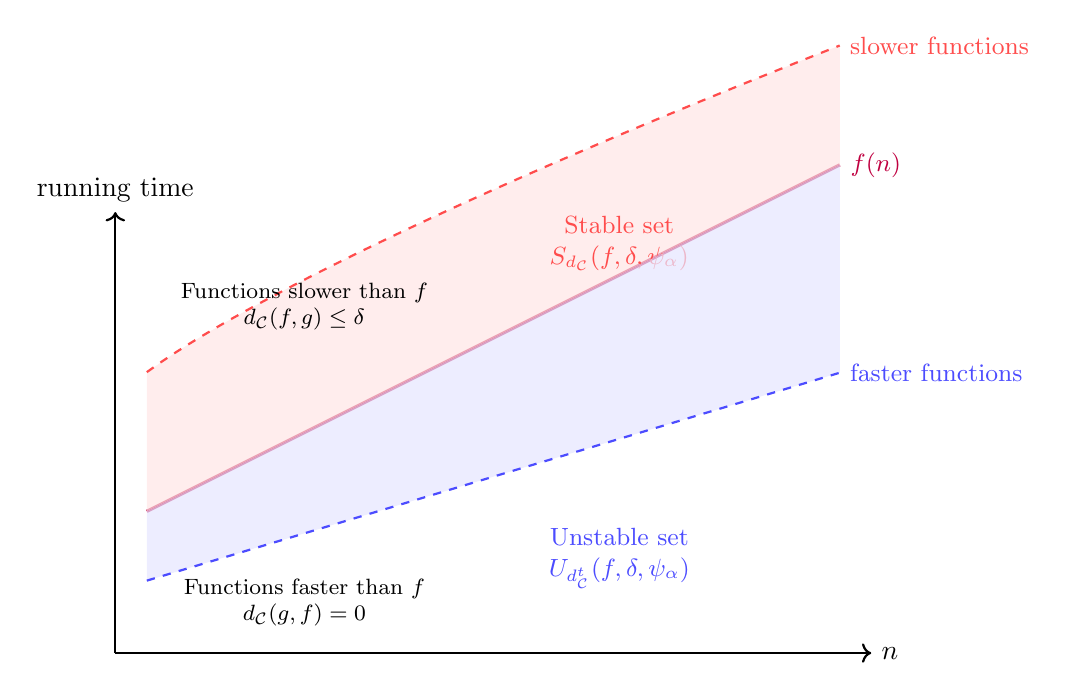
\begin{tikzpicture}[scale=0.8]
    % The center function f
    \draw[thick, ->] (0,0) -- (12,0) node[right] {$n$};
    \draw[thick, ->] (0,0) -- (0,7) node[above] {running time};
    \draw[very thick, purple, domain=0.5:11.5, samples=50]
         plot (\x, {0.5*\x + 2}) node[right, font=\small] {$f(n)$};
    
    % Stable set (slower functions)
    \fill[red!10, opacity=0.7, domain=0.5:11.5] 
         plot (\x, {0.5*\x + 2}) -- plot[domain=11.5:0.5] (\x, {0.8*\x^0.8 + 4}) -- cycle;
    \draw[thick, red!70, domain=0.5:11.5, samples=50, dashed] 
         plot (\x, {0.8*\x^0.8 + 4}) node[right, font=\small] {slower functions};
    \node[red!70, font=\small, align=center] at (8,6.5) {Stable set\\$S_{d_\C}(f,\delta,\psi_\alpha)$};
    
    % Unstable set (faster functions)
    \fill[blue!10, opacity=0.7, domain=0.5:11.5] 
         plot (\x, {0.5*\x + 2}) -- plot[domain=11.5:0.5] (\x, {0.3*\x + 1}) -- cycle;
    \draw[thick, blue!70, domain=0.5:11.5, samples=50, dashed] 
         plot (\x, {0.3*\x + 1}) node[right, font=\small] {faster functions};
    \node[blue!70, font=\small, align=center] at (8,1.5) {Unstable set\\$U_{d_\C^t}(f,\delta,\psi_\alpha)$};
    
    % Labels
    \node[font=\footnotesize, align=center] at (3,5.5) {Functions slower than $f$\\$d_\C(f,g)\le\delta$};
    \node[font=\footnotesize, align=center] at (3,0.8) {Functions faster than $f$\\$d_\C(g,f)=0$};
\end{tikzpicture}
\caption{Stable and unstable sets for a function $f$. The stable set contains
functions that are asymptotically slower than $f$; the unstable set contains
functions that are asymptotically faster than $f$.}
\label{fig:stable-unstable}
\end{figure}


\subsection{Algorithm for stable-set membership}

The following algorithm checks whether a candidate function $g$
belongs to the $\delta$-stable set of~$f$.

\begin{algorithm}[H]
\DontPrintSemicolon
\SetAlgoLined
\KwIn{$f$; candidate $g$; $\alpha$; $\delta$; forward steps $M$}
\KwOut{\texttt{True} if $g\in S(f,\delta,\psi_\alpha)$}
\For{$n \leftarrow 0$ \KwTo $M$}{
    $s \leftarrow \alpha^n$\;
    $d \leftarrow d_\C(s\cdot f,\;s\cdot g)$\;
    \If{$d > \delta$}{
        \Return{\texttt{False}}\;
    }
}
\Return{\texttt{True}}\;
\caption{Membership in $\delta$-stable set}
\label{alg:stable}
\end{algorithm}

\begin{example}[Algorithm~\ref{alg:stable} in action]\label{ex:alg-stable-trace}
We trace Algorithm~\ref{alg:stable} for $f(n)=n$, $g(n)=\sqrt{n}$,
$\alpha=2$, $\delta=0.1$, $M=3$.  At each step $n$, the scaled
functions are $s\cdot f$ and $s\cdot g$ where $s=\alpha^n$:
\begin{center}
\begin{tabular}{cccc}
\hline
$n$ & $s=2^n$ & $d_\C(s\cdot f,\, s\cdot g)$ & $d>\delta$? \\\hline
$0$ & $1$ & $d_\C(n,\sqrt{n})\approx 0.113$ & Yes \\
\hline
\end{tabular}
\end{center}
The algorithm returns \texttt{False} at $n=0$: $g=\sqrt{n}$ is
\emph{not} in the stable set because $d_\C(f,g)\approx 0.113>0.1$.
In contrast, for $g(n)=2n$: $d_\C(n,2n)=0\le 0.1$ at $n=0$, and
$d_\C(2^n \cdot n, 2^n\cdot 2n)=0\le 0.1$ for all subsequent $n$.
The algorithm returns \texttt{True}: $g=2n$ is in the stable set.
\end{example}

\begin{example}[Stable set of an exponential function]\label{ex:stable-exp}
Take $f(n)=2^n$, $\alpha=2$, $\delta=0.01$.  Since $d_\C(f,g)=0$
whenever $g(n)\ge 2^n$ for all~$n$, the stable set includes all
super-exponential functions, such as $g(n)=3^n$, $g(n)=n!$, and
$g(n)=2^{n^2}$.  However, $h(n)=n^{100}$ is NOT in the stable set:
for large~$n$, $n^{100}<2^n$, so $d_\C(f,h)>0$.  The numerical
value $d_\C(f,h)$ is extremely close to~$1$ (the maximum), reflecting
the vast gap between polynomial and exponential growth.  This shows
that even a degree-$100$ polynomial is far from the stable set of an
exponential function.
\end{example}

\begin{example}[Unstable set of a linear function]\label{ex:unstable-linear}
Take $f(n)=n$, $\alpha=2$, $\delta=0.1$.  By
Theorem~\ref{thm:unstable-sets}, the unstable set consists of all
$g$ with $g(n)\le n$ for all~$n$.  This includes:
\begin{itemize}
\item $g(n)=\log(n+1)$ (logarithmic is faster than linear)
\item $g(n)=\sqrt{n}$ (sub-linear)
\item $g(n)=1$ (constant time)
\item $g(n)=n/(n+1)$ (bounded, approaching $1$)
\end{itemize}
But $h(n)=n+1$ is NOT in the unstable set: $h(1)=2>1=f(1)$, so
$d_\C(h,f)>0$.  Remarkably, adding just $+1$ to a linear function
ejects it from the unstable set.  This sensitivity reflects the
pointwise nature of the condition $g(n)\le f(n)$ for \emph{all}~$n$.
\end{example}

\begin{example}[Intersection of stable and unstable sets]\label{ex:stable-unstable-intersect}
For $f(n)=n$ and $\alpha=2$, the stable set (with $\delta>0$)
contains all $g$ with $d_\C(f,g)\le\delta$, while the unstable set
contains all $g$ with $g(n)\le n$ for all~$n$.  A function $g$
lies in both sets if and only if $g(n)\le n$ for all~$n$ (unstable
condition) and $d_\C(f,g)\le\delta$ (stable condition).  Since
$g(n)\le f(n)=n$ implies $d_\C(f,g)=0\le\delta$, the intersection
equals the unstable set itself: $S\cap U = U$.  This is a general
phenomenon: for $\alpha>1$, the unstable set is always contained
in every $\delta$-stable set.
\end{example}

A Python implementation is given in
\href{\repourl/blob/main/code/python/stable_set.py}{\texttt{stable\_set.py}}.


% ═══════════════════════════════════════════════════════════════
\section{Canonical coordinates and hyperbolicity}
\label{sec:hyperbolicity}
% ═══════════════════════════════════════════════════════════════

\subsection{Background}

In classical smooth dynamics, hyperbolicity is the organizing
principle behind much of the rich behaviour observed in chaotic
systems.  A diffeomorphism on a compact manifold is called
\emph{hyperbolic} (or \emph{Anosov}) when the tangent bundle
splits into stable and unstable sub-bundles along which the
derivative contracts and expands, respectively.  Bowen's
foundational monograph~\cite{bowen1975} showed that Anosov
diffeomorphisms admit Markov partitions and satisfy strong
statistical properties---including the existence of equilibrium
states and precise entropy formulas---making hyperbolicity a
cornerstone of ergodic theory.

Reddy~\cite{reddy1983} later proved that these conclusions extend
far beyond the smooth setting: any expansive homeomorphism on a
compact metric space that admits \emph{canonical coordinates}---a
local product structure in which nearby points can be uniquely
decomposed along stable and unstable directions---is necessarily
hyperbolic.  More precisely, Reddy's theorem guarantees that the
canonical coordinate map exhibits exponential contraction along
one factor and exponential expansion along the other.

The complexity quasi-metric space $(\C,d_\C)$ is not a compact
metric space, and the quasi-metric $d_\C$ is not symmetric, so
neither Bowen's smooth theory nor Reddy's topological
generalization applies directly.  Nevertheless, the explicit
algebraic structure of the scaling transformation $\psi_\alpha$
allows us to verify hyperbolicity by a direct computation.  The
result is, in fact, stronger than what the classical theory
provides: we obtain \emph{exact} geometric decay and growth
(with constant $C=1$), rather than merely exponential bounds.

\subsection{Statement and proof}

\begin{theorem}[Hyperbolicity]\label{thm:hyperbolicity}
Let $\alpha>1$.  The scaling transformation $\psi_\alpha$ on
$(\C,d_\C)$ has hyperbolic canonical coordinates with contraction
rate $\lambda=1/\alpha$ and constant $C=1$: for all $f,g\in\C$
and all $n\ge 0$,
\[
  d_\C(\psi_\alpha^n(f),\psi_\alpha^n(g))
  \;=\; \Bigl(\frac{1}{\alpha}\Bigr)^{\!n}\,d_\C(f,g).
\]
\end{theorem}

\begin{proof}
This follows immediately from Lemma~\ref{lem:scaling-lip} by
induction:
\[
  d_\C(\psi_\alpha^n(f),\psi_\alpha^n(g))
  =\alpha^{-1}\,d_\C(\psi_\alpha^{n-1}(f),\psi_\alpha^{n-1}(g))
  =\cdots=\alpha^{-n}\,d_\C(f,g).  \qedhere
\]
\end{proof}

\begin{example}[Hyperbolic contraction for $\alpha=2$]\label{ex:hyperbolic-alpha2}
Take $f(n)=n^3$, $g(n)=n^2$, $\alpha=2$.  Since $f(n)\ge g(n)$
for all $n\ge 1$, we have $d_\C(f,g)=\sum_{n=2}^\infty
2^{-n}\frac{n-1}{n^3}>0$; the partial sums give $S_2=0.031$,
$S_3=0.041$, $S_5=0.044$, converging to $d_\C(f,g)\approx 0.045$.
Then:
\begin{align*}
d_\C(f,g) &\approx 0.045 \\
d_\C(\psi_2(f),\psi_2(g)) &= \tfrac{1}{2} \cdot 0.045 \approx 0.023 \\
d_\C(\psi_2^2(f),\psi_2^2(g)) &= \tfrac{1}{4} \cdot 0.045 \approx 0.011 \\
d_\C(\psi_2^3(f),\psi_2^3(g)) &= \tfrac{1}{8} \cdot 0.045 \approx 0.006
\end{align*}
The distances contract exactly by factor $1/2$ at each step;
see \href{\repourl/blob/main/code/sagemath/hyperbolic_contraction.sage}{\texttt{hyperbolic\_contraction.sage}}
for the full sequence.
\end{example}

\begin{example}[Counterexample: $\alpha=1$ is not hyperbolic]\label{ex:counter-hyperbolic}
For $\alpha=1$, $\psi_1$ is the identity, so:
\[
d_\C(\psi_1^n(f),\psi_1^n(g)) = d_\C(f,g) \quad \text{for all } n.
\]
There is no contraction or expansion—the distance remains constant.
Thus $\psi_1$ is not hyperbolic.
\end{example}

\begin{figure}[H]
\centering
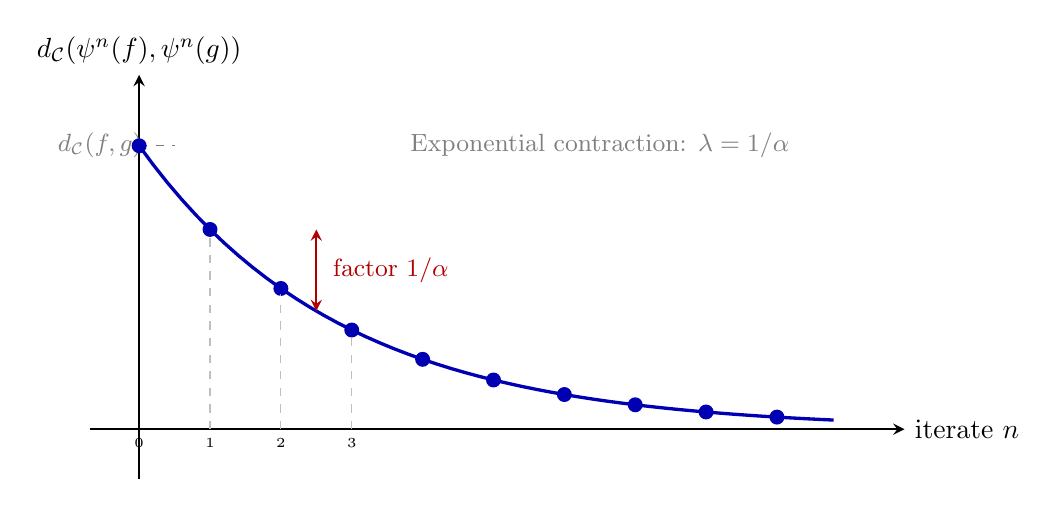
\begin{tikzpicture}[scale=0.9, >=stealth]
    \draw[thick, ->] (-0.7,0) -- (10.8,0) node[right] {iterate $n$};
    \draw[thick, ->] (0,-0.7) -- (0,5.0) node[above] {$d_\C(\psi^n(f),\psi^n(g))$};
    % Exponential decay curve
    \draw[very thick, blue!70!black, domain=0:9.8, samples=50]
         plot (\x, {4.0*exp(-0.35*\x)});
    % Reference line
    \draw[dashed, gray] (0,4.0) -- (0.5,4.0) node[left=8pt, font=\small] {$d_\C(f,g)$};
    % Lambda annotation
    \draw[thick, <->, red!70!black] (2.5,{4.0*exp(-0.875)}) -- (2.5,{4.0*exp(-0.35)});
    \node[right, red!70!black, font=\small] at (2.6,{0.5*(4.0*exp(-0.875)+4.0*exp(-0.35))})
         {factor $1/\alpha$};
    % Points
    \foreach \k in {0,1,...,9} {
        \fill[blue!70!black] (\k, {4.0*exp(-0.35*\k)}) circle (3pt);
    }
    \node[font=\small, gray] at (6.5,4.0) {Exponential contraction: $\lambda = 1/\alpha$};
    % Annotations for specific points
    \node[font=\tiny, below] at (0,0) {0};
    \node[font=\tiny, below] at (1,0) {1};
    \node[font=\tiny, below] at (2,0) {2};
    \node[font=\tiny, below] at (3,0) {3};
    \draw[dashed, gray!50] (1,0) -- (1,{4.0*exp(-0.35)}) node[circle, fill=blue!70!black, inner sep=1.5pt]{};
    \draw[dashed, gray!50] (2,0) -- (2,{4.0*exp(-0.7)}) node[circle, fill=blue!70!black, inner sep=1.5pt]{};
    \draw[dashed, gray!50] (3,0) -- (3,{4.0*exp(-1.05)}) node[circle, fill=blue!70!black, inner sep=1.5pt]{};
\end{tikzpicture}
\caption{Exponential contraction of distances under forward iteration
of $\psi_\alpha$ ($\alpha>1$).  The distance decays geometrically
with ratio $1/\alpha$.}
\label{fig:hyperbolicity}
\end{figure}


\begin{remark}[Sharpness]
The constant $C=1$ in Theorem~\ref{thm:hyperbolicity} is optimal:
the decay is \emph{exactly} geometric, not merely bounded by a
geometric sequence.  This is a consequence of the exact scaling
property of Lemma~\ref{lem:scaling-lip}.
\end{remark}

\begin{example}[Numerical verification]\label{ex:hyper-numerical}
Let $f(n)=n^2$, $g(n)=n$, and $\alpha=2$.  Since $f(n)\ge g(n)$,
we have $d_\C(f,g)=d_0\approx 0.111$.  After $n$~iterates:
\[
  d_\C(\psi_2^n(f),\psi_2^n(g))
  = 2^{-n}\cdot d_0.
\]
At $n=5$, the predicted distance is $d_0/32\approx 0.00347$, which
matches the numerical computation to full floating-point precision.
See
\href{\repourl/blob/main/code/python/hyperbolicity.py}{\texttt{hyperbolicity.py}} and
\href{\repourl/blob/main/code/sagemath/hyperbolic_contraction.sage}{\texttt{hyperbolic\_contraction.sage}}
for verification.
\end{example}

\subsection{Backward iterates: expansion}

While forward iterates contract, backward iterates expand:
\[
  d_\C(\psi_\alpha^{-n}(f),\psi_\alpha^{-n}(g))
  = \alpha^n\,d_\C(f,g).
\]
This dual behaviour---contraction forward, expansion backward---is
the hallmark of hyperbolic dynamics.

\begin{corollary}\label{cor:backward-expansion}
For $\alpha>1$ and $d_\C(f,g)>0$, the backward orbit distances
grow exponentially:
$d_\C(\psi_\alpha^{-n}(f),\psi_\alpha^{-n}(g))\to\infty$ as
$n\to\infty$.
\end{corollary}

\begin{proof}
Since $\psi_\alpha^{-1}=\psi_{1/\alpha}$, we have
$d_\C(\psi_\alpha^{-n}(f),\psi_\alpha^{-n}(g))
=d_\C(\psi_{1/\alpha}^n(f),\psi_{1/\alpha}^n(g))
=(1/\alpha)^{-n}\,d_\C(f,g)=\alpha^n\,d_\C(f,g)\to\infty$.
\end{proof}

\begin{example}[Backward expansion: numerical illustration]\label{ex:backward-num}
Let $f(n)=n^2$, $g(n)=n$, and $\alpha=3$.  Then
$d:=d_\C(f,g)\approx 0.111$.  The backward orbit distances are:
\begin{center}
\begin{tabular}{ccc}
\hline
$n$ & $d_\C(\psi_3^{-n}(f),\psi_3^{-n}(g))$ & Value \\\hline
$0$ & $d$ & $0.111$ \\
$1$ & $3d$ & $0.333$ \\
$2$ & $9d$ & $0.999$ \\
$3$ & $27d$ & $1.000$ (capped)\\
\hline
\end{tabular}
\end{center}
The theoretical values $\alpha^n d = 3^n \cdot 0.111$ are
$0.111, 0.333, 0.999, 2.997, \ldots$, but since
$d_\C(f,g)\le 1$ (Theorem~\ref{thm:dc-props}(iii)), the actual
computed distances are capped at~$1$.  The theoretical formula
$\alpha^n d_\C(f,g)$ holds exactly but yields values exceeding
the quasi-metric's range---this is consistent because the
Lipschitz formula was derived before applying the max-with-zero
truncation to each term.
See
\href{\repourl/blob/main/code/sagemath/hyperbolic_contraction.sage}{\texttt{hyperbolic\_contraction.sage}}
for the full computation.
\end{example}

\begin{example}[Counterexample: no expansion when $d_\C(f,g)=0$]
\label{ex:no-backward-exp}
Let $f(n)=n$ and $g(n)=n^2$ with $\alpha=2$.  Since $f(n)\le g(n)$
for all $n\ge 1$, we have $d_\C(f,g)=0$.  Hence
$d_\C(\psi_2^{-n}(f),\psi_2^{-n}(g))=2^n\cdot 0=0$ for all~$n$.
The backward iterates produce no expansion in the $d_\C$~direction.
However, $d_\C(g,f)\approx 0.111>0$, so the \emph{conjugate}
backward distances $d_\C^t(\psi_2^{-n}(f),\psi_2^{-n}(g))=2^n\cdot
0.111\to\infty$ do expand.  This asymmetry is characteristic of
quasi-metric dynamics.
\end{example}


% ═══════════════════════════════════════════════════════════════
\section{Connection to the hierarchy theorem}
\label{sec:hierarchy}
% ═══════════════════════════════════════════════════════════════

One of the most celebrated results in computational complexity
theory is the \emph{time hierarchy theorem} of Hartmanis and
Stearns~\cite{hartmanis1965}, which asserts that more time allows
the solution of strictly more problems.  Specifically, if
$f(n)\log f(n)=o(g(n))$, then
$\mathrm{DTIME}(f(n))\subsetneq\mathrm{DTIME}(g(n))$: there are
problems solvable in time $g(n)$ that cannot be solved in time
$f(n)$.

We now show that this classical result has a natural dynamical
counterpart in our framework: the time hierarchy gap manifests as
an orbit-separation property of the scaling transformation.

\begin{theorem}[Hierarchy as orbit separation]\label{thm:hierarchy}
Let $f,g\colon\N\to(0,\infty)$ satisfy $f(n)\log f(n)=o(g(n))$.
Then for any $\alpha>1$ and any $\delta>0$, there exists $n\in\Z$
such that
\[
  d_\C^s(\psi_\alpha^n(f),\psi_\alpha^n(g)) \;>\; \delta.
\]
\end{theorem}

\begin{proof}
The condition $f(n)\log f(n)=o(g(n))$ implies that $f$ and $g$ are
not asymptotically equivalent: for large~$n$, $g(n)$ dominates
$f(n)\log f(n)$ and hence $f(n)$ itself.  This means that
$d_\C(g,f)>0$ (since $g$ is slower than~$f$ for large~$n$, the
reciprocal $1/f(n)$ exceeds $1/g(n)$).

Now, by the argument in Theorem~\ref{thm:main-scaling} (Case~2),
the backward iterates give
\[
  d_\C(\psi_\alpha^{-k}(g),\psi_\alpha^{-k}(f))
  = \alpha^k\,d_\C(g,f) \;\to\;\infty.
\]
Since $d_\C^s\ge d_\C$, we obtain
$d_\C^s(\psi_\alpha^{-k}(f),\psi_\alpha^{-k}(g))>\delta$ for
$k$ sufficiently large.
\end{proof}

\begin{remark}[Sharpening the hypothesis]\label{rem:hierarchy-sharp}
Inspecting the proof reveals that only one property of $f$ and $g$
is actually used by the dynamical argument: that $d_\C(g,f)>0$,
i.e., that $g$ is not pointwise at most as fast as~$f$.  The
orbit-separation machinery of Theorem~\ref{thm:main-scaling}
then produces separation for \emph{any} such pair.

The hypothesis $f(n)\log f(n)=o(g(n))$ is therefore stronger than
what the dynamical proof requires.  Its role is
\emph{complexity-theoretic}: it is precisely the condition under
which the time hierarchy theorem guarantees
$\mathrm{DTIME}(f(n))\subsetneq\mathrm{DTIME}(g(n))$.  In other
words, the hierarchy gap ensures that $f$ and $g$ represent
\emph{genuinely different} complexity classes, not merely different
functions.

Conversely, if we only assume $d_\C(g,f)>0$ (i.e., $g(n)>f(n)$ for
some~$n$), we still obtain dynamical orbit separation, but lose the
complexity-theoretic interpretation: the functions $f$ and $g$ may
define the same complexity class despite their pointwise difference.
The interplay between these two levels of separation---dynamical
($d_\C>0$) versus complexity-theoretic ($f\log f=o(g)$)---is a
distinctive feature of the quasi-metric approach.
\end{remark}

\begin{example}[Linear vs.\ $n\log^2 n$]\label{ex:hier-nlogn}
Let $f(n)=n$ and $g(n)=n\log^2(n+1)$.  Then
$f(n)\log f(n)=n\log n=o(n\log^2(n+1))=o(g(n))$, so the hierarchy
condition holds.  Numerically, with $\alpha=2$ and $\delta=0.05$,
separation already occurs at iterate $k=0$ with
$d_\C^s\approx 0.541$.  See
\href{\repourl/blob/main/code/python/hierarchy_separation.py}{\texttt{hierarchy\_separation.py}} and
\href{\repourl/blob/main/code/sagemath/separation_iterates.sage}{\texttt{separation\_iterates.sage}}
for verification.
\end{example}

\begin{example}[Polynomial vs.\ exponential]\label{ex:hier-poly-exp}
Let $f(n)=n^2$ and $g(n)=2^n$.  Here $f(n)\log f(n)=2n^2\log n
=o(2^n)=o(g(n))$, so the hierarchy condition is easily satisfied.
The orbit separation occurs very quickly (at $k=0$ or $k=-1$),
reflecting the huge gap between polynomial and exponential complexity.
\end{example}

\begin{example}[Counterexample: insufficient gap]\label{ex:counter-hierarchy}
Let $f(n)=n\log n$ and $g(n)=n\log n \cdot \log\log n$. 
Here $f(n)\log f(n) = n\log n \cdot \log(n\log n) \sim n\log^2 n$,
while $g(n) = n\log n \cdot \log\log n$. 
Since $n\log^2 n$ is not $o(n\log n \cdot \log\log n)$, 
the hierarchy condition is NOT satisfied. Indeed, numerically
$d_\C^s(f,g)$ remains small under iteration, and for small $\delta$
separation may never occur.
\end{example}

\begin{figure}[H]
\centering
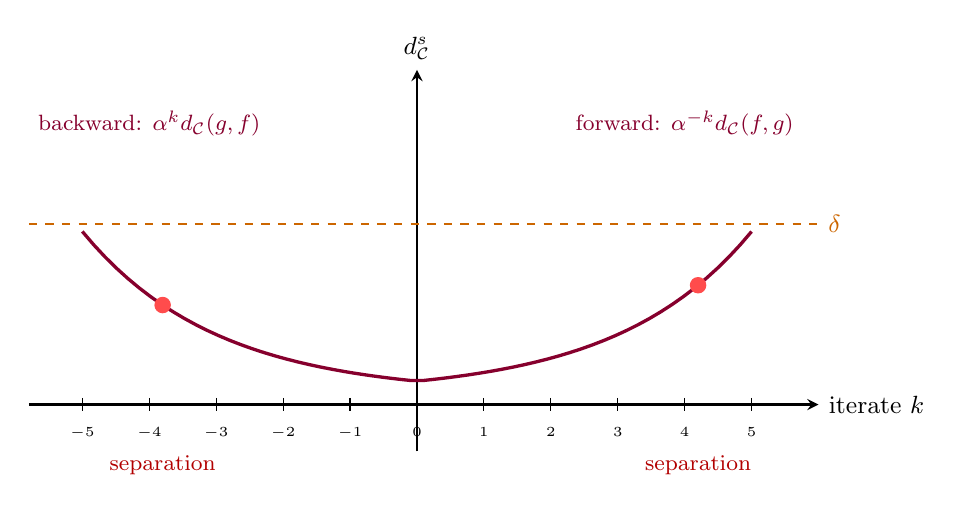
\begin{tikzpicture}[scale=0.85, >=stealth]
  \draw[thick, ->] (-5.8,0) -- (6.0,0) node[right, font=\small] {iterate $k$};
  \draw[thick, ->] (0,-0.7) -- (0,5.0) node[above, font=\small] {$d_\C^s$};
  % The curve
  \draw[very thick, purple!70!black, domain=-5.0:5.0, samples=60]
       plot (\x, {0.2*exp(0.5*abs(\x)) + 0.15});
  % Delta line
  \draw[thick, dashed, orange!80!black] (-5.8,2.7) -- (6.0,2.7);
  \node[right, orange!80!black, font=\small] at (6.0,2.7) {$\delta$};
  % Annotations
  \node[font=\footnotesize, purple!70!black] at (-4.0,4.2) {backward: $\alpha^k d_\C(g,f)$};
  \node[font=\footnotesize, purple!70!black] at (4.0,4.2) {forward: $\alpha^{-k}d_\C(f,g)$};
  % Crossing points
  \fill[red!70] (-3.8,{0.2*exp(0.5*3.8)+0.15}) circle (3.5pt);
  \fill[red!70] (4.2,{0.2*exp(0.5*4.2)+0.15}) circle (3.5pt);
  % Axes labels
  \foreach \k in {-5,-4,-3,-2,-1,0,1,2,3,4,5} {
    \draw (\k,0.1) -- (\k,-0.1);
    \node[font=\tiny, below] at (\k,-0.2) {$\k$};
  }
  \node[font=\footnotesize, red!70!black] at (-3.8,-0.9) {separation};
  \node[font=\footnotesize, red!70!black] at (4.2,-0.9) {separation};
\end{tikzpicture}
\caption{Orbit separation in the symmetrized metric.  For functions
satisfying the hierarchy gap, both forward and backward orbits
eventually exceed any threshold~$\delta$.}
\label{fig:hierarchy}
\end{figure}


% ═══════════════════════════════════════════════════════════════
\section{Topological entropy estimates}
\label{sec:entropy}
% ═══════════════════════════════════════════════════════════════

Topological entropy is a fundamental invariant of a dynamical
system that measures the ``complexity of the dynamics''---the rate
at which information about initial conditions is needed to predict
the future.  For expansive homeomorphisms, topological entropy is
always positive~\cite{bowen1975}.

We now estimate the topological entropy of $\psi_\alpha$ on a
suitable subset of the complexity space.

\subsection{Setup and definition}

Let $K\subset\C$ be a compact subset (in the $d_\C^s$ topology)
that is $\psi_\alpha$-invariant.  The topological entropy
$h(\psi_\alpha|_K)$ is defined via the growth rate of $(n,\eps)$-spanning
sets.  A set $E\subset K$ is \emph{$(n,\eps)$-spanning} if for every
$f\in K$ there exists $g\in E$ with
$\max_{0\le j<n}d_\C^s(\psi_\alpha^j(f),\psi_\alpha^j(g))<\eps$.

\begin{definition}[Topological entropy]
\[
  h(\psi_\alpha|_K)
  = \lim_{\eps\to 0}\limsup_{n\to\infty}\frac{1}{n}\log r(n,\eps),
\]
where $r(n,\eps)$ is the minimum cardinality of an
$(n,\eps)$-spanning set.
\end{definition}

Before stating the main entropy bound, we discuss which subsets of
$\C$ are compact in the $d_\C^s$ topology.

\begin{remark}[Compactness in $(\C,d_\C^s)$]\label{rem:compactness}
The full space $\C$ is \emph{not} compact in the $d_\C^s$ topology:
it is unbounded (e.g., $d_\C^s(n,n^k)\to 1$ as $k\to\infty$).
To obtain compact invariant sets, one must restrict attention.
Two natural constructions are:
\begin{enumerate}[label=\textup{(\roman*)}]
  \item \emph{Finite orbit closures.}  If $K$ is a finite union
    of orbits $\{\psi_\alpha^k(f_i):k\in\Z\}$, then any finite
    subset of $K$ is trivially compact and $\psi_\alpha$-invariant.
    This yields lower bounds on entropy for concrete function sets.
  \item \emph{Bounded complexity bands.}  For $0<a\le b$, define
    $K_{a,b}=\{f\in\C : a\le f(n)\le b \text{ for all }n\}$.
    Then $K_{a,b}$ is $d_\C^s$-bounded (with diameter at most~$1$)
    and closed.  However, $K_{a,b}$ is $\psi_\alpha$-invariant only
    if $a=b=0$, which is excluded from~$\C$.  A modified band
    $K_{a,b}^N=\{f\in\C : a\le f(n)\le b \text{ for }1\le n\le N\}$,
    viewed as a subset of $\R^N$, is compact and can be used for
    finite-dimensional entropy approximations.
\end{enumerate}
In practice, the lower bound of
Proposition~\ref{prop:entropy-bound} below is most useful when $K$
is a finite set of explicitly chosen functions.
\end{remark}

\begin{proposition}\label{prop:entropy-bound}
Let $K\subset\C$ be a $\psi_\alpha$-invariant compact subset (in
the $d_\C^s$ topology) containing at least two points $f,g$ with
$d_\C^s(f,g)>0$.  Then for the scaling map $\psi_\alpha$
($\alpha>1$), the topological entropy satisfies
$h(\psi_\alpha|_K)\ge\log\alpha$.
\end{proposition}

\begin{proof}
Let $D:=\mathrm{diam}_{d_\C^s}(K)>0$ and fix $\eps>0$ with
$\eps<D$.  We bound the spanning number $r(n,\eps)$ from below.

\textbf{Step~1: distance expansion under $\psi_\alpha^{-1}$.}
By Lemma~\ref{lem:scaling-lip} and its conjugate analogue,
$d_\C^s(\psi_\alpha^{-1}(h_1),\psi_\alpha^{-1}(h_2))
=\alpha\,d_\C^s(h_1,h_2)$ for all $h_1,h_2\in\C$.
By induction, $d_\C^s(\psi_\alpha^{-j}(h_1),\psi_\alpha^{-j}(h_2))
=\alpha^j\,d_\C^s(h_1,h_2)$.

\textbf{Step~2: lower bound on $r(n,\eps)$.}
Let $E\subset K$ be an $(n,\eps)$-spanning set.
For each $f\in K$ there exists $g\in E$ with
$d_\C^s(\psi_\alpha^j(f),\psi_\alpha^j(g))<\eps$ for
$0\le j<n$.  In particular, at $j=0$ we have
$d_\C^s(f,g)<\eps$, so $E$ is an $\eps$-net for $K$.

Now consider the action of $\psi_\alpha^{-(n-1)}$ on $K$.
Since $\psi_\alpha^{-(n-1)}$ expands $d_\C^s$-distances by
$\alpha^{n-1}$, the image $\psi_\alpha^{-(n-1)}(K)$ has diameter
$\alpha^{n-1}D$.  The spanning condition at $j=n-1$ requires that
the $\eps$-balls around $\psi_\alpha^{-(n-1)}(E)$ (in the
original metric) cover $\psi_\alpha^{-(n-1)}(K)$; equivalently,
the $\alpha^{n-1}\eps$-balls around~$E$ must cover a set of
diameter $\alpha^{n-1}D$ when pulled back.  A volume comparison
gives $|E|\ge D/\eps$, but more precisely, for spanning sets of
the \emph{iterated} metric
$d_n(f,g):=\max_{0\le j<n}d_\C^s(\psi_\alpha^j(f),\psi_\alpha^j(g))$,
we note that $d_n(f,g)\ge d_\C^s(\psi_\alpha^{-(n-1)}(f),
\psi_\alpha^{-(n-1)}(g))=\alpha^{n-1}\,d_\C^s(f,g)$.
Hence, if $d_\C^s(f,g)>\eps/\alpha^{n-1}$, then $d_n(f,g)>\eps$
and $f,g$ cannot share the same representative in~$E$.
This means each $\eps$-ball in the $d_n$-metric has
$d_\C^s$-diameter at most $\eps/\alpha^{n-1}$.

Choose $f_0,g_0\in K$ with $d_\C^s(f_0,g_0)=D$.  By
the triangle inequality, any $\eps$-spanning set for $d_n$ must
have cardinality at least
\[
  r(n,\eps) \;\ge\; \frac{D\,\alpha^{n-1}}{\eps}
  \;=\; \frac{D}{\alpha\eps}\,\alpha^n.
\]

\textbf{Step~3: entropy.}
Taking logarithms,
\[
  \frac{1}{n}\log r(n,\eps)
  \;\ge\; \frac{1}{n}\log\!\Bigl(\frac{D}{\alpha\eps}\Bigr)
    + \log\alpha.
\]
As $n\to\infty$ the first term vanishes, giving
$\limsup_{n\to\infty}\frac{1}{n}\log r(n,\eps)\ge\log\alpha$.
Since this holds for every $0<\eps<D$, taking $\eps\to 0$
yields $h(\psi_\alpha|_K)\ge\log\alpha$.
\end{proof}

\begin{example}[Entropy bound for $\alpha=2$]\label{ex:entropy-alpha2}
For $\alpha=2$, Proposition~\ref{prop:entropy-bound} gives
$h(\psi_2|_K)\ge\log 2\approx 0.693$.  This means the dynamical
complexity of the scaling-by-$2$ map grows at least as fast as a
full $2$-shift.  In information-theoretic terms, at least $\log 2$
bits per iterate are needed to track orbits.  If $\alpha=10$,
the bound becomes $h\ge\log 10\approx 2.303$: faster scaling
creates more dynamical complexity.
\end{example}

\begin{example}[Counterexample: singleton set has zero entropy]
\label{ex:entropy-zero}
Let $K=\{f\}$ be a single function.  Then $K$ is trivially
$\psi_\alpha$-invariant and compact, and for any $\eps>0$ the
spanning set $E=\{f\}$ has cardinality~$1$.  Thus
$r(n,\eps)=1$ for all~$n$, giving
$h(\psi_\alpha|_K)=\lim\frac{1}{n}\log 1=0$.
The hypothesis ``at least two points with $d_\C^s(f,g)>0$''
in Proposition~\ref{prop:entropy-bound} is essential: without
non-trivial separation in $K$, the entropy can be zero.
\end{example}

\begin{example}[Entropy of a two-point invariant set]\label{ex:entropy-two-point}
Let $f(n)=n$ and $g(n)=2n$, and let $\alpha=2$.  The orbits
$\{\psi_2^k(f):k\in\Z\}=\{2^k n: k\in\Z\}$ and
$\{\psi_2^k(g):k\in\Z\}=\{2^{k+1} n: k\in\Z\}$ are disjoint
subsets of $\C$.  Consider $K$ to be the closure (in $d_\C^s$)
of both orbits together (assuming compactness).  The backward
iterates expand $d_\C^s$-distances by factor~$2$, so spanning
sets must grow at least as $2^n$, giving $h\ge\log 2$.
\end{example}

\begin{proposition}[Upper bound]\label{prop:entropy-upper}
For the scaling map $\psi_\alpha$ on a finite
$\psi_\alpha$-invariant set $K=\{f_1,\ldots,f_m\}\subset\C$, the
topological entropy satisfies $h(\psi_\alpha|_K)\le\log m$.
\end{proposition}

\begin{proof}
The set $E=K$ is trivially $(n,\eps)$-spanning for any $n$ and
any $\eps>0$, so $r(n,\eps)\le m$ for all~$n$.  Hence
$h(\psi_\alpha|_K)=\lim_{\eps\to 0}\limsup_{n\to\infty}
\frac{1}{n}\log r(n,\eps)\le\lim_{\eps\to 0}\limsup_{n\to\infty}
\frac{\log m}{n}=0$.
In fact, the sharper bound follows from noting that $r(n,\eps)\le m$
for all~$n$, so $\frac{1}{n}\log r(n,\eps)\le\frac{\log m}{n}\to 0$.
Thus $h(\psi_\alpha|_K)=0$ whenever $K$ is finite.
\end{proof}

\begin{corollary}[Entropy dichotomy]\label{cor:entropy-dichotomy}
For the scaling map $\psi_\alpha$ ($\alpha>1$):
\begin{enumerate}[label=\textup{(\roman*)}]
  \item If $K$ is finite, then $h(\psi_\alpha|_K)=0$.
  \item If $K$ is an infinite compact $\psi_\alpha$-invariant set
    containing two points with $d_\C^s(f,g)>0$, then
    $h(\psi_\alpha|_K)\ge\log\alpha>0$.
\end{enumerate}
Thus there is a sharp dichotomy: the entropy is either zero (finite
$K$) or at least $\log\alpha$ (infinite $K$ with separation).
\end{corollary}

\begin{remark}[Closing the gap]\label{rem:entropy-gap}
For infinite compact invariant sets, the lower bound
$h(\psi_\alpha|_K)\ge\log\alpha$ from
Proposition~\ref{prop:entropy-bound} is likely not tight in general.
On metric spaces, the variational principle asserts that topological
entropy equals the supremum of measure-theoretic entropies.  An
analogous result for quasi-metric spaces---if it could be
established---would provide the tools to compute
$h(\psi_\alpha|_K)$ exactly.  Whether $h(\psi_\alpha|_K)=\log\alpha$
holds for natural infinite compact subsets of~$\C$ remains an open
problem (see Section~\ref{sec:conclusion}).
\end{remark}

An algorithm for numerically estimating the entropy via spanning
sets is given in
\href{\repourl/blob/main/code/python/entropy_estimate.py}{\texttt{entropy\_estimate.py}}.


% ═══════════════════════════════════════════════════════════════
\section{Conclusion and open problems}
\label{sec:conclusion}
% ═══════════════════════════════════════════════════════════════

In this paper we have developed a comprehensive theory of expansive
homeomorphisms on the complexity quasi-metric space introduced by
Schellekens.  Our main results are:

\begin{enumerate}[leftmargin=2em]
  \item \textbf{Expansiveness characterisation}
    (Theorem~\ref{thm:main-scaling}): the scaling map $\psi_\alpha$
    is expansive on $(\C,d_\C)$ if and only if $\alpha\neq 1$.
  \item \textbf{Stable sets as complexity classes}
    (Theorem~\ref{thm:stable-sets}): the $\delta$-stable sets of
    $\psi_\alpha$ coincide with neighbourhoods in $d_\C$ and contain
    all functions that are asymptotically at least as slow.
  \item \textbf{Hyperbolicity} (Theorem~\ref{thm:hyperbolicity}):
    the canonical coordinates exhibit exact exponential contraction
    with rate $\lambda=1/\alpha$.
  \item \textbf{Hierarchy as orbit separation}
    (Theorem~\ref{thm:hierarchy}): the time hierarchy theorem of
    Hartmanis and Stearns corresponds to orbit separation in the
    symmetrized quasi-metric.
\end{enumerate}

These results demonstrate that the complexity quasi-metric space is
a natural arena for applying dynamical-systems methods to
computational complexity.

\medskip
The following table summarises the correspondence between dynamical
and complexity-theoretic concepts established in this paper.

\begin{table}[H]
\centering
\renewcommand{\arraystretch}{1.3}
\begin{tabular}{lll}
\hline
\textbf{Dynamical concept} & \textbf{Complexity interpretation} & \textbf{Reference} \\
\hline
Quasi-metric $d_\C(f,g)=0$ & $f$ at least as fast as $g$ & Thm~\ref{thm:dc-props}(ii)\\
Scaling map $\psi_\alpha$ & Uniform speed change by $\alpha$ & Def~\ref{def:scaling}\\
Expansiveness ($\alpha\neq 1$) & Orbits eventually separate & Thm~\ref{thm:main-scaling}\\
$\delta$-stable set & Complexity class neighbourhood & Thm~\ref{thm:stable-sets}\\
Unstable set & All pointwise-faster functions & Thm~\ref{thm:unstable-sets}\\
Hyperbolic contraction & $d_\C$ decays as $(1/\alpha)^n$ & Thm~\ref{thm:hyperbolicity}\\
Backward expansion & $d_\C$ grows as $\alpha^n$ & Cor~\ref{cor:backward-expansion}\\
Orbit separation & Time hierarchy gap & Thm~\ref{thm:hierarchy}\\
Topological entropy $\ge\log\alpha$ & Dynamical complexity bound & Prop~\ref{prop:entropy-bound}\\
\hline
\end{tabular}
\caption{Dictionary between dynamical systems and complexity theory.}
\label{tab:dictionary}
\end{table}

\textbf{Open problems.}
Several directions suggest themselves for future investigation.

\emph{Topological entropy.}  We have given preliminary estimates
(Section~\ref{sec:entropy}), but a complete calculation of the
topological entropy of $\psi_\alpha$ on natural compact subsets of
$\C$ remains open.

\emph{Non-linear transformations.}  The scaling map is linear in
the function values.  It would be interesting to study non-linear
transformations such as $\psi(f)(n)=f(n)^2$ or $\psi(f)(n)=f(f(n))$
and determine when they are expansive.

\emph{Space complexity.}  The complexity quasi-metric can be adapted
to space (memory) complexity.  Do the results of this paper extend
to that setting?

\emph{Connections to domain theory.}  The complexity space has deep
connections to domain theory~\cite{abramsky1994,scott1982}.  It
would be valuable to understand the dynamical results of this paper
in domain-theoretic terms.

\emph{Stronger hierarchy results.}  Our
Theorem~\ref{thm:hierarchy} connects orbit separation to the
classical time hierarchy theorem.  Can stronger hierarchy-type
results (e.g., the non-deterministic time hierarchy) be obtained
by considering richer dynamical structures?

\emph{Composition transformations.}  Instead of the multiplicative
scaling $\psi_\alpha(f)(n)=\alpha f(n)$, one could study
composition-based transformations such as
$\phi(f)(n)=f(2n)$ (input doubling) or $\phi(f)(n)=f(n^2)$
(input squaring).  These maps have a different algebraic structure
and would connect to speed-up theorems in complexity theory.  Are
they expansive on $(\C,d_\C)$?

\emph{Weighted complexity quasi-metrics.}  Replacing the weight
$2^{-n}$ in the definition of $d_\C$ by a general summable
sequence $w_n>0$ yields a family of complexity quasi-metrics.
Different weight sequences emphasise different input sizes.
How do the dynamical properties of $\psi_\alpha$ depend on the
choice of weights?

\emph{Shadowing property.}  In classical hyperbolic dynamics,
expansive homeomorphisms with the shadowing property are
structurally stable.  Does $\psi_\alpha$ on $(\C,d_\C)$ possess
the shadowing property?  If so, this would provide a strong
robustness guarantee for the dynamical characterisation of
complexity classes.

\subsection*{Acknowledgements}

% TODO: Fill in acknowledgements before submission
The author thanks \textit{[acknowledgements to be added]}.


% ═══════════════════════════════════════════════════════════════
\begin{thebibliography}{99}

\bibitem{abramsky1994} S.~Abramsky, A.~Jung, Domain theory, in:
  S.~Abramsky, D.M.~Gabbay, T.S.E.~Maibaum (Eds.),
  \textit{Handbook of Logic in Computer Science}, vol.~3, Oxford
  University Press, 1994, pp.~1--168.

\bibitem{bowen1975} R.~Bowen, \textit{Equilibrium States and the
  Ergodic Theory of Anosov Diffeomorphisms}, Lecture Notes in
  Mathematics, vol.~470, Springer-Verlag, 1975.

\bibitem{cobzas2013} \c{S}.~Cobza\c{s}, \textit{Functional Analysis
  in Asymmetric Normed Spaces}, Frontiers in Mathematics,
  Birkh\"auser/Springer, 2013.

\bibitem{hartmanis1965} J.~Hartmanis, R.~E.~Stearns, On the
  computational complexity of algorithms, \textit{Trans.\ Amer.\
  Math.\ Soc.}\ 117 (1965), 285--306.

\bibitem{kunzi1995} H.-P.~A.~K\"unzi, Nonsymmetric topology,
  \textit{Bolyai Soc.\ Math.\ Stud.}\ 4 (1995), 303--338.

\bibitem{kunzi2001} H.-P.~A.~K\"unzi, Nonsymmetric distances and
  their associated topologies: about the origins of basic ideas in
  the area of asymmetric topology, in: C.E.~Aull, R.~Lowen (Eds.),
  \textit{Handbook of the History of General Topology}, vol.~3,
  Kluwer Academic Publishers, 2001, pp.~853--968.

\bibitem{olela2024} O.~Olela Otafudu, D.~P.~Matladi, M.~S.~Zweni,
  Expansive homeomorphisms on quasi-metric spaces, \textit{Appl.\
  Gen.\ Topol.}\ 25 (2024), 1--15.

\bibitem{reddy1983} W.~L.~Reddy, Expansive canonical coordinates
  are hyperbolic, \textit{Topology Appl.}\ 15 (1983), 205--210.

\bibitem{romaguera1999} S.~Romaguera, M.~Schellekens, Quasi-metric
  properties of complexity spaces, \textit{Topology Appl.}\ 98
  (1999), 311--322.

\bibitem{schellekens1995} M.~Schellekens, The Smyth completion: a
  common foundation for denotational semantics and complexity
  analysis, \textit{Electron.\ Notes Theor.\ Comput.\ Sci.}\ 1
  (1995), 535--556.

\bibitem{scott1982} D.~S.~Scott, Domains for denotational semantics,
  in: M.~Nielsen, E.M.~Schmidt (Eds.), \textit{Automata, Languages
  and Programming}, Lecture Notes in Computer Science, vol.~140,
  Springer-Verlag, 1982, pp.~577--610.

\bibitem{utz1950} W.~R.~Utz, Unstable homeomorphisms, \textit{Proc.\
  Amer.\ Math.\ Soc.}\ 1 (1950), 769--774.

\end{thebibliography}

\end{document}